\documentclass{template/socthesis}

\usepackage{subcaption}
\usepackage{amsmath}
\usepackage{enumitem}
\usepackage{color} % balíček pro obarvování textů
\usepackage{xcolor}  % zapne možnost používání barev, mj. pro \definecolor
\definecolor{mygreen}{RGB}{0,150,0} % nastavení barev odkazů 
\usepackage{listings} % balíček pro formátování zdrojových kódů 
\usepackage[author=,status=draft]{fixme} % vkládání poznámek  
% dva módy (status): draft (poznámky se zobrazují v PDF) / final (poznámky se nezobrazují v PDF)
\usepackage{multirow}
\usepackage{pifont}
\usepackage{hyperref}

\newcommand{\cmark}{\textcolor{green}{\ding{51}}}
\newcommand{\xmark}{\textcolor{red}{\ding{55}}}

\addbibresource{text.bib}
\nocite{*}

\titlecz{Automatický skleník}
\titleen{Automatic greenhouse}
\author{Petr Štourač}
\field{10}
\school{Střední průmyslová škola a Vyšší odborná škola Brno, Sokolská, příspěvková organizace}  

\mentor{Mgr. Miroslav Burda}
\mentorstatement{Mgr. Miroslava Burdy}



% Změňte, pokud se liší
%\region{Jihomoravský}
%\placefooter{Brno 2018}

\begin{document}
	
	\maketitle
	
	\makecopyrightstatement{V~Brně}
	
	\makethanks{Děkuji svému školiteli Mgr. Miroslavu Burdovi za obětavou pomoc, podnětné připomínky a nekonečnou trpělivost, kterou mi během práce poskytoval. Zároveň děkuji svému otci za samotný námět práce a paní profesorce Mgr.~Janě Vaculíkové za korekci anglického textu.}
	
	\pagestyle{empty}
	
	\section*{Anotace}

    Pěstování skleníkových rostlin je velice roz\-ší\-řenou činností.
	Lidé, kteří běžně chodí do práce, mají stále méně času na péči o svoje skleníkové rostliny.
	Mojí snahou je těmto lidem péči o~rostliny částečně usnadnit zautomatizováním každodenních činností, jako je zalévání nebo větrání.
	
	Mým řešením je systém na automatizaci skleníku s~názvem ProtoPlant.
	Celý systém je navržen tak, aby byl jednoduchý na obsluhu, byl modulární a~zároveň levný. 
	Po instalaci jej uživatel spustí, provede prvotní nastavení 
	a~o~zbytek se již ProtoPlant postará sám.
	
	\subsection*{Klíčová slova}
	automatický skleník; automatizace; zavlažování; ventilace; skleníkové rostliny
		
	\section*{Annotation}
    Growing greenhouse plants is a very common hobby.
    People, who must work every day simply have less and less time to care about their greenhouse plants.
    My endeavour is to help these people by automating everyday actions, such as irrigation, or ventilation.
	
	My solution of this problem is ProtoPlant, greenhouse automation system.
	Whole system is designed to be simple, modular and cheap.
	After installation, user goes through the first time setup and from this point, Protoplants begins to take care of everything else alone.
	
	\subsection*{Keywords}
	automatic greenhouse; automation; irrigation; ventilation; greenhouse plants
	
	\newpage
	\pagestyle{plain}
	
    \tableofcontents % vysází obsah
	
	%%% Začátek práce
	\setcounter{figure}{0}
	\setcounter{table}{0}
	\newpage
	
	%%% Úvod
	\chapter*{Úvod}
\addcontentsline{toc}{chapter}{Úvod} % přidá položku úvod do obsahu

Pěstování skleníkových rostlin, ať již okrasných, či užitkových, je velice roz\-ší\-řenou činností, pokud o ní mluvíme jako o činnosti zájmové.
Ovšem tato činnost je i velice časově náročná.
Lidé, kteří běžně chodí do práce mají stále méně času na péči o svoje skleníkové rostliny.
Mojí snahou je těmto lidem péči o rostliny částečně usnadnit zautomatizováním každodenních činností, jako je zalévání nebo větrání.

Mým řešením je systém na automatizaci skleníku s názvem ProtoPlant \cite{protoPlantWeb}.
Celý systém je navržen tak, aby byl jednoduchý na obsluhu, modulární a zároveň levný.
Po instalaci jej uživatel spustí, provede prvotní nastavení a o zbytek se již ProtoPlant postará sám.

Nabídka komerčních řešení je v tomto ohledu velmi chudá.
Samořejmě, existují průmyslová řešení, ovšem ta jsou určena pro firmy, nikoliv pro jednotlivce, jsou tedy velmi drahá.
Na webu existují návody na automatizaci skleníku, ovšem ty jsou určeny pro osoby, které již mají s elektrotechnikou nějaké zkušenosti, opět tedy jen pro užší skupinu lidí.

Při návrhu ProtoPlantu jsem dbal na to, aby měl několik důležitých vlastností:
\begin{itemize}
    \item jednoduchost používání a obsluhy -- chci, aby byl systém jednoduchý svojí obsluhou
    \item modularita -- celý systém je složen z modulů, které se dají jednoduše spojovat
    \item nízká cena -- chci, aby systém byl dostupný, jak cenově, tak i materiálně
    \item univerzálnost -- systém použitelný pro širokou škálu rostlin a plodin
    \item samostatnost -- systém se dokáže o sebe postarat sám po určitou dobu
    \item jednoduchá instalace -- uživatel dokáže ProtoPlant nainstalovat sám
\end{itemize}

Tyto vlastnosti jej činí ideálním pro použití v běžné domácnosti.

\newpage


	%%% Motivace
	\chapter{Proč automatický skleník?}
K~samotnému nápadu na automatizaci skleníku mě dovedl můj otec, který vlastní skleník s orchidejemi.
Z časových důvodů hledal způsob, jak zautomatizovat běžné operace, na které sám neměl čas.
Na trhu ovšem neexistuje žádné univerzální řešení, dostupné pro běžné uživatele.
Jsou různá průmyslová řešení pro automatizaci skleníku.
Jejich instalace se ale provádí na míru pro velkozemědělské společnosti.
Zároveň jsou velmi drahá.
Samozřejmě, existuje i mnoho různých návodů na automatizaci skleníku s použitím Arduina, ovšem realizace vyžaduje určité znalosti v oblasti programování a elektroniky, tudíž takové řešení opět není vhodné pro všechny. 
Proto mě napadlo vytvořit ProtoPlant -- systém, dostupný téměř všem. Jediným předpokladem by bylo vlastnit skleník. Do něj uživatel pouze nainstaluje elektroniku a rozvody vody, které poté napojí na můj systém.


	%%% Srovnani
	\chapter{Srovnání s konkurencí}
Co se týče konkurence ProtoPlantu, řadí se do dvou kategorií:
\begin{itemize} 
    \item průmyslová řešení
    \item řešení vytvořená kutily
\end{itemize}

\section{Průmyslová řešení}
V případě průmyslových řešení existují různé možnosti.
Ovšem prakticky všechny z nich jsou určeny pro využití ve velkých sklenících používaných ve velkozemědělství.
Zároveň je valná většina z nich instalována na míru -- není zde tedy možnost toho, že by si tento systém uživatel nainstaloval sám.

Co se ceny týče, ta se u~těchto systémů šplhá až do stovek tisíc, chybí zde tedy i cenová dostupnost těchto systémů.

Samotné řízení těchto průmyslových systémů je v drtivé většině případů zajišťováno tzv. PLC -- programovatelnými automaty.
Samotné PLC jsou velmi drahá a fungují jen čistě jakožto řídící hardware -- senzory a periferie tedy nejsou do ceny započítány.

Několik příkladů používaných PLC v tabulce \ref{table:plc_pricing}.
\begin{table}
    \centering
    \caption{Srovnání PLC a ProtoPLant řídící jednotky}
    \begin{tabular}{lllll}
    PLC        & Cena     & Výrobce       & Síťové vybavení & Příslušenství 
    (senzory, atp.)     \\
    \hline
    MPC 410\cite{MicropelPLC}    & 7 300,- & Micropel      & není            & \multirow{4}{*}{Nutné dokoupit }  \\
    S7 - 1200\cite{S7-1200PLC}   & 7 825,-   & Siement       & Ethernet        &                                   \\
    FX3s\cite{FX3sPLC}           & 6 000,-   & Mitsubishi    & Ethernet        &                                   \\
    Micro 810\cite{Micro810PLC}  & 2 693,-   & Allen Bradley & není            &                                   \\
    \hline
    ProtoPlant                   & 2 000,-   &               & WiFi, bluetooth & Senzory, napájení v ceně         
    \end{tabular}
    \label{table:plc_pricing}
    \end{table}

U dalšího hardwaru to je s cenou velmi podobné.
Firmy navíc dělají tyto instalace na zakázku, tudíž je třeba si připlatit i za práci.

\section{Kutilská řešení}
U~této kategorie sice konkurence existuje, ovšem projekty, které jsem našel na webu postrádají několik vlastností ProtoPlantu.

Tyto vlastnosti jsou:
\begin{itemize}
    \item jednoduchost -- k výrobě jsou třeba zkušenosti s elektrotechnikou
    \item univerzálnost -- většina těchto řešení je určena pro malé skleníky
    \item modularita
\end{itemize}

Daly by se sice nazvat cenově příznivé, ovšem co se týče dostupnosti, jsou tyto projekty vhodné pouze pro uživatele, kteří mají určité znalosti s~programováním a~elektrotechnikou.

Pro srovnání uvedu dva příklady.
\subsection{Arduino: automatický skleník}
Autor této bakalářské práce \cite{sklenikVavra} se přede mnou již pokusil vytvořit systém podobný ProtoPlantu založený na Arduinu.
Jde ovšem pouze o teoretickou práci, jeho systém nikdy nebyl uveden do praxe.

\subsection{Raspberry Pi Greenhouse}
Tento projekt \cite{raspPIgreenhouse} je založen na Raspberry PI.
Nutností pro jeho sestavení jsou určité znalosti v elektrotechnice a programování.

\begin{table}[]
    \centering
    \caption{Srovnání ProtoPlantu a projektu s RPI}
    \begin{tabular}{lll}
    Vlastnost                                                            & ProtoPlant                  & Projekt s Raspberry PI \\ \hline
    \multicolumn{1}{l|}{Modularita}                                      & \multicolumn{1}{l|}{\cmark} & \xmark                 \\
    \multicolumn{1}{l|}{Univerzálnost}                                   & \multicolumn{1}{l|}{\cmark} & \xmark                 \\
    \multicolumn{1}{l|}{Jednoduchost instalace}                          & \multicolumn{1}{l|}{\cmark} & \xmark                 \\
    \multicolumn{1}{l|}{Uvedení do praktického provozu}                  & \multicolumn{1}{l|}{\cmark} & \cmark                 \\
    \multicolumn{1}{l|}{Možnost instalace do různých velikostí skleníku} & \multicolumn{1}{l|}{\cmark} & \xmark                 \\
    \multicolumn{1}{l|}{Odolnost (vodotěsnost)}                          & \multicolumn{1}{l|}{\cmark} & \xmark                 \\
    \multicolumn{1}{l|}{Cena}                                            & \multicolumn{1}{l|}{\cmark} & \cmark                
    \label{table:comparationPPandRPI}
    \end{tabular}
    \end{table}

\section{Shrnutí}
Konkurence v~tomto oboru je skutečně chudá.
Na jedné straně jsou drahá průmyslová řešení instalovaná na míru, na straně druhé jsou tu projekty pro kutily, které ovšem jsou určeny jen pro uživatele se znalostí elektrotechniky a~programování.
Tuto díru na trhu se snažím vyplnit vytvořením ProtoPlantu -- systému dostupnému pro běžné uživatele a~domácnosti, který bude dostupný i~cenově i~materiálně.


	%%% Hardware
	\chapter{Hardware}
Jak již bylo zmíněno, ProtoPlant je modulární systém.
Jádrem celého systému je řídící jednotka. 
K~ní jsou připojeny periferie, jako senzory, čerpadla, atd.

\section{Napájení}
Systém je rozdělen na celkem 2 napájecí okruhy.
Zdrojem el. proudu je zásuvka.
Do ní se s pomocí klasické vidlicové zástrčky připojí měniče první a druhé větve.
První větev s napětím 12~V je používaná k~napájení aktuátorů.
Druhá, 5-ti~voltová větev napájí řídící elektroniku a senzory.

%\fxnote*[author=MB]{místo 3.3 patří 3,3 V}{obrázek}

\section{Řídící jednotka}
Jádrem celého systému je tzv. řídící jednotka.
Vnější obal tvoří vodotěsná průmyslová krabice z~ABS plastu s~krytím IP65.
Ta v sobě ukrývá řídící elektroniku a~invertor polarity (viz. níže).
Na krajích řídící jednotky se nachází průchodky s~kabelovými vývody pro připojení ostatního hardwaru.
Na přední straně se nachází znakový lcd display (20x4) a několik průmyslových tlačítek sloužících k ručnímu ovládání zavlažování a oken.

\subsection{ESP32 DevKit C}
Celý systém je řízen touto deskou, která je osazena mikroprocesorem ESP32. 
Celá deska má celkem 37 pinů, z toho jeden napájecí a dva zemnící. 
16 pinů lze použít jako analogové.

Důvod, proč jsem se rozhodl své řešení založit na ESP32 DevKitu C je jednoduchý.
Deska je univerzální, má poměrně dobrý výkon a sama o sobě podporuje WiFi, čímž je možno systém vylepšit o možnost ovládání přes internet, když jsme například na dovolené. 

Samotná deska je určena pro napájení 5~V, je tedy připojena k druhé napájecí větvi.

\subsection{Invertor polarity pro pohon oken}
Toto zařízení slouží k měnění polarity lineárních aktuátorů používaných pro otevírání a zavírání oken.
Sestává se ze tří spínacích relé, z nichž jedno řídí napájení a zbylá dvě slouží k inverzi polarity.

Princip zařízení je jednoduchý.
Jakmile je nutné otevřít/zavřít okna, je nejdříve sepnuto relé, které řídí napájení.
V případě otevírání se dále sepnou obě relé řídící polaritu -- okna se začnou zavírat.
Pro dobu běhu motoru je stanoven fixní časový limit, který závisí na délce aktuátorů a jejich rychlosti. Po jeho uběhnutí se napájecí relé opět rozepne a aktuátory tedy přestanou být napájeny.
Zároveň se rozepne i relé řídící polaritu.
Jakmile chceme okna zavřít, relé řídící polaritu zůstanou rozepnuta a sepne jen relé ovládající napájení.



%\fxnote*[author=MB]{Text "Relé 3" nejde přečíst}{obrázek}
\section{Aktuátory pro manipulaci s okny}
Pro otevírání a zavírání oken používám lineární aktuátory.
Jejich pracovní napětí je 12~V.
Samotné aktuátory mají zabudovaná koncová čidla, po dojezdu do koncové polohy se samy zastaví.
Směr jejich pohybu lze ovládat inverzí polarity, kterou vykonává můj invertor polarity umístěný v řídící jednotce.

\section{Senzory}
Ke sledování stavu prostředí ve skleníku používám několik senzorů.
\begin{itemize}
	\item DHT 11, případně DHT 22
	\item DS18B20
\end{itemize}

\subsection{DHT 11/22}
DHT 11/22 jsou čidla, která používám pro měření vlhkosti vzduchu.
Jsou určena pro napájení na 5~V stejnosměrného napětí.
Jsou rozmístěna na krajích skleníku, z naměřených hodnot je následně vytvořen průměr. 
Počet použitých čidel se liší podle velikosti skleníku, ovšem pro základní verzi ProtoPlantu je z důvodu nedostatku GPIO u ESP32 nastaven limit tři senzory. Dva vnitřní a~jeden venkovní.

\subsection{DS18B20}
Tyto senzory používám k měření teploty.
Jsou zapojena přes 1-Wire sběrnici, což umožňuje připojení maximálně 10 těchto senzorů k jednomu pinu.
Samotný senzor má 3 piny: jeden napájecí (VCC), druhý datový (DQ) a třetí pro společnou zem napájecí i datovou (GND).
1-Wire sběrnice dokáže pracovat ve dvou režimech napájení senzorů, klasickém třídrátovém, nebo v režimu napájení parazitního (s využitím jen dvou drátů).
Z těchto dvou režimů využívá ProtoPlant režim klasický, třídrátový režim.

Maximální počet těchto senzorů, který je možno připojit k systému ProtoPlant je omezen na 6.

\section{Ovládání oken}
Okna jsou ovládána lineárními elektro-mechanickými aktuátory.
Jejich provozní napětí je 12~V.
Díky využití stejnosměrných motorů je možno měnit směr jejich pohybu jednoduchým obrácením polarity, což zajišťuje invertor polarity popsaný výše.
Rychlost posuvu je fixní, doba vysunutí tedy závisí pouze na délce aktuátorů.

\section{Ventilátor}
Pro zlepšení regulace vzdušné vlhkosti a zlepšení cirkulace vzduchu využívám pro drobnou korekci teploty ventilátor připevněný na stěně skleníku.
Ten se spustí v době, kdy je vnitřní teplota velmi nízko nad nastavenou horní mezí.

\section{Zavlažování}
Zavlažování obstarává vysokotlaké čerpadlo vody, které nasává vodu z nádrže umístěné přímo ve skleníku.
Je napájeno 12~V stejnosměrného napětí.
Čerpadlo je řízeno s pomocí SSR relé umístěného v řídící jednotce.
Voda se čerpá do rozvodů umístěných v horní části skleníku.
Na těchto rozvodech jsou nainstalovány rozprašovače.



%\fxnote*[author=MB]{Na obrázku je použito 220V místo 230V}{obrázek}

	
	%%% Software
	\chapter{Software a popis funkce}
Tato kapitola se týká popisu funkce celého systému ProtoPlant a softwarové stránky projektu.

\section{ProtoPlant knihovna}
Softwarová knihovna PPlant vytvořená mnou obsahuje jednodušší podpůrné funkce ovládající hardware skleníku.
Mezi ně patří:
\begin{itemize}
    \item Spouštění a zastavování čerpadla vody
    \item Práce s LCD
\end{itemize}

\section{Start-up sekvence}
Tato sekvence se sestává z několika operací nutných pro správnou inicializaci systému.

Celá sekvence by se dala rozdělit na několik úkonů:
\begin{enumerate}
    \item Inicializace LCD
    \item Kontrola systému
    \item Inicializace senzorů
    \item Nastavení krajních hodnot parametrů prostředí, nebo jejich načtení z paměti
\end{enumerate}
Po dokončení celé sekvence se systém automaticky přepne do režimu standby, ve kterém na pozadí monitoruje vlhkost a teplotu.

\subsection{První spuštění}
Při prvním spuštění se systém při provádění startup sekvence zastaví v bodě 4, při kterém musí uživatel nastavit krajní hodnoty vlhkosti a teploty.
Ty uloží následně do flash paměti čipu ESP32, kde zůstanou zachované i v případě, že se systém vypne, nebo vypadne proud.
Po zadání a~uložení hodnot systém následně pokračuje v běhu přechodem do režimu standby.

\subsection{Opakované spuštění}
Při opakovaném spuštění již systém v bodě 4 nastavení parametrů nepožaduje, místo toho si načte uložené hodnoty z paměti a pokračuje v normálním chodu.

\section{Režim STANDBY}
Po proběhnutí startup sekvence se systém automaticky přepne do režimu STANDBY.
V tomto režimu systém na pozadí periodicky měří hodnoty vlhkosti a teploty, které následně porovnává s~hodnotami uloženými ve flash paměti.
Zároveň naměřené hodnoty vypíše na LCD~displej.

\section{Zavlažování a měření vlhkosti}
Vlhkost vzduchu je pravidelně měřena třemi senzory DHT22 rozmístěnými po skleníku. %\fxnote*[author=MB]{Výše píšete o maximálně dvou}{několika}
Interval pro měření teploty je nastaven na 1 minutu, což je optimální doba vypozorovaná z testování, které jsem dříve provedl.
Z dat naměřených jednotlivými senzory je následně vypočten aritmetický průměr.
Výsledná hodnota je porovnaná s krajními mezemi vlhkosti nastavenými uživatelem.
Pokud je výsledek v mezích, skleník pokračuje v~periodickém měření vlhkosti. Pokud je vlhkost příliš nízká, systém sepne solid state relé umístěné v řídící jednotce. 
Čerpadlo, které je k němu připojené se tedy spustí. 
%\fxnote*[author=MB]{A co když je ve skleníku moc vlhko?}{v mezích},
V případě, že je vlhkost příliš vysoká, systém otevře okna, případně spustí ventilátor umístěný na stěně skleníku.

\subsection{Softwarová stránka zavlažování}
Zavlažování je po softwarové stránce velmi jednoduchým úkonem.
Měření a zpracování teploty zajišťují knihovny DHT a DHT\_U přímo od výrobce senzorů DHT22, Adafruitu.
Samotné porovnání teploty s mezní hodnotou je provedeno v hlavním programu main. 
Spouštění čerpadla se následně provede zavoláním příkazu pro spuštění čerpadla, který obsaženého v knihovně PPlant.

\section{Ovládání oken}
Systém v pravidelných intervalech měří teplotu.
Tuto naměřenou hodnotu porovnanává s mezními hodnotami uloženými v paměti.
V případě, že je teplota v mezích, systém pokračuje v normálním chodu.
Pokud je teplota příliš vysoká, okna se otevřou, pokud je teplota moc nízká, zavřou se.

\subsection{Software pro ovládání oken}
Pro řízení inventoru polarity aktuátorů ovládajících okna jsem napsal vlastní knihovnu.
% Celá je řízena těmito pěti  \fxnote*[author=MB]{Více v poznámce ve zdrojovém textu }{funkcemi.}
\begin{verbatim}  Mezi některé funkce této knihovny patří:
    window.begin();         
    window.getstate();      
    window.close();         
    window.open();          
    window.changestate();
\end{verbatim}

%pro formátování kódu doporučuju balíček listings, viz https://en.wikibooks.org/wiki/LaTeX/Source_Code_Listings
% například: \lstinputlisting{priklady_c/blikani_LED1.cpp}
% a nebo alespoň písmo verbatim \verb@"psací stroj"@

Nejdříve se knihovna inicializuje zavoláním funkce window.begin();.
Funkce getstate(); je využívána pro zjištění, zda jsou okna otevřená, či nikoliv. 
Jejím výstupem je logická hodnota true/false.
Funkce open(); a close(); jsou využity, jak již jejich název napovídá k otevření, či zavření oken.
S pomocí funkce changestate(); jsme schopni přepínat mezi otevřeným/zavřeným stavem nezávisle na tom, jakém stavu jsou před jejím zavoláním.
V případě, že jsou okna před jejím zavoláním otevřená, zavolání funkce je zavře a naopak.


	
	%%% Velká verze skleníku
	\chapter{Velká verze skleníku}
Celý systém testuji ve skleníku mého otce, ve kterém pěstuje orchideje.
V celém skleníku jsou nainstalovány rozvody vody i elektrického proudu.
Těsně pod stropem skleníku jsou rozvedeny trubice, na kterých jsou nainstalovány rozprašovače, slouží tedy k zavlažování.
Pro ovládání oken jsou zde nainstalovány lineární aktuátory popsané v sekci 1.2.2 s délkou výsuvu 45 cm.
Samotný skleník je umístěn z části pod zemí, z důvodu snížení nákladů na vytápění.
Pod úrovní podlahy je umístěna nádrž na vodu s kapacitou 3,5~m$^3$ pro použití při zavlažování.
Do této nádrže je sbírána dešťová voda z okapů.

Co se týče senzorů, v této plné verzi jsou instalovány 3 senzory DHT i 3 DS18B20.
Ty jsou rovnoměrně rozmístěny tak, aby bylo pokrytí jejich měření rozloženo po celém skleníku.
Jsou připevněna na kabelech visících ze stropu skleníku.

Verze systému 1.0 byla dokončena teprve nedávno, připravuji tedy nasazení pro testovací provoz v tomto skleníku.
Co se týče mých očekávání, předpokládám, že výsledkem testu bude značná úspora práce.
Dále očekávám úsporu tepla i~energií, vzhledem k tomu, že se bude větrat pouze, pokud to bude nutné.




 %\color{mygreen}
%[MB:] Chybí údaje o testovacím provozu: 
%\begin{itemize}
	%\item jak dlouho testování probíhá ?
	%\item s jakými výsledky (úspora tepla, vody, práce ... ) jak velká?
	%\item kolik je jakých čidel a kde jsou osazená? 
	%\item  jaká byla spolehlivost provozu? 
	%\item  Jaké byly náklady pro uvedení do provozu? 
	%\item  Jak velká je nádrž a odkud se bere voda? Je přívod taky automatický? 
	
%\end{itemize}
 %\color{black}


	%%% Malá verze skleníku
	\chapter{Prezentační model}
Pro ilustraci jak celý systém funguje, jsem vytvořil funkční model skleníku o rozměrech 1000x500x400~mm.
Jeho základem je běžný pařník, který lze zakoupit v jakémkoliv zahradnictví.
Do něj jsem nainstaloval velmi podobný hardware jako do velké verze.
Co se týče řídící jednotky, je totožná s~verzí nainstalovanou ve velkém skleníku.
Beze změny využívám i~stejné senzory, stykač a čerpadlo.
Okna jsou ovládána aktuátory stejného typu, jako ve velké verzi, jen s kratší délkou výsuvu, která činí 4", tedy přibližně 10~cm.
Kvůli jeho menší velikosti je počet senzorů DS18B20 i DHT 11/22 snížen na dva, které jsou umístěné tesně nad trubicí pro zavlažování.

Tento prezentační model je plně funkční, tudíž je možné jej použít i jako samostatnou jednotku pro péči o rostliny v domácnostech.

Náklady na uvedení této verze skleníku do chodu jsou rozepsány v tabulce~\ref{table:small_greenhouse_pricing_full} na straně 
\pageref{table:small_greenhouse_pricing_full}.

\begin{table}
	\centering
	\caption{Celková cena kompletní malé verze skleníku}
	\begin{tabular}{llll}
	Položka         				& Cena / položka & Počet & Celk. cena  \\ 
	\hline
	Pařník          				& 780,-          & 1     & 780,-       \\
	Aktuátory       				& 1090,-         & 2     & 2180,-      \\
	Řídící jednotka + zákl. moduly 	& 1500,-         & 1     & 1500,-      \\ 
	\hline
	Celkem         				 	&                &       & 4460,-      
	\label{table:small_greenhouse_pricing_full}
	\end{tabular}
	\end{table}

Dále je možné pořídit pouze tzv. upgrade kit -- set na vylepšení běžného skleníku. Jeho cena je uvedena v tabulce \ref{table:small_greenhouse_pricing_upgrade} na straně \pageref{table:small_greenhouse_pricing_upgrade}.

\begin{table}
	\centering
	\caption{Celková cena upgrade kitu pro malý skleník}
	\begin{tabular}{llll}
	Položka         				& Cena / položka & Počet & Celk. cena  \\ 
	\hline
	Aktuátory       				& 1090,-         & 2     & 2180,-      \\
	Řídící jednotka + zákl. moduly 	& 1500,-         & 1     & 1500,-      \\ 
	\hline
	Celkem          				&                &       & 3680,-     
	\label{table:small_greenhouse_pricing_upgrade}
	\end{tabular}
	\end{table}

	
	%%% Závěr
	\chapter*{Závěr}
\addcontentsline{toc}{chapter}{Závěr}

Mojí hlavní prioritou při tvorbě této práce byla snaha pomoct lidem, kteří vlastní skleník, ale nemají dostatek času se o něj starat.
V momentálním stavu je systém schopen automaticky otevírat okna, provádět zavlažování, měřit teplotu a vlhkost.
Možnosti využití jsou široké, vzhledem k tomu, že je systém univerzální a použitelný pro široký okruh rostlin, ať již okrasných, či užitkových.
Věřím, že právě díky univerzálnosti celého systému a poměrně nízké ceně si své využití najde především u široké veřejnosti.

Dále bych rád ProtoPlant rozvíjel po stránce možnosti skleník vzdáleně ovládat, případně kontrolovat přes internet například z dovolené.
V Internetu věcí vidím velké možnosti dalšího rozvoje.
Zároveň bych rád vylepšil i software skleníku a implementoval další funkce včetně možnosti záznamu změn teplot a generování grafů z těchto hodnot.

Co se týče cílů, o těch mohu říct, že jsem je splnil.
Podařilo se mi vytvořit systém pro automatizaci skleníku, který je univerzální, modulární, samostatný, jednoduše se instaluje a ovládá a je cenově dostupný.

Novinky z vývoje můžete sledovat na webových stránkách \\ www.protoplant.stpindustries.cz.

% \color{mygreen}
%[MB:] Vím, že Vás vůbec nešetřím... 
%\begin{itemize}
%	\item  Bude příloha se zdrojovými kódy vašeho software? Nebo alespoň vývojový a nebo stavový  diagram? 
%	\item  Jsme v kategorii elekro: bude nějaké schéma systému v Eaglu a pod.? 
%	\item  V přílohách by určitě měly být fotografie jak z velkého skleníku, tak modelu. 
%	\item  Chybí použitá literatura a odkazy, včetně datasheetů použitých modulů, srovnání s konkurencí, a pod. - probereme osobně/telefonicky 
	
%\end{itemize}
%\color{black}




	
	\newpage


	\printbibliography[title=Literatura]
	\addcontentsline{toc}{section}{Literatura}
	
	\listoffigures
	\addcontentsline{toc}{section}{Seznam obrázků}
	
	\listoftables
	\addcontentsline{toc}{section}{Seznam tabulek}
	
%	\listoflistedequation
%	\addcontentsline{toc}{section}{Seznam rovnic}
\chapter*{Přílohy}
\addcontentsline{toc}{chapter}{Přílohy}

\begin{figure}[htbp]
    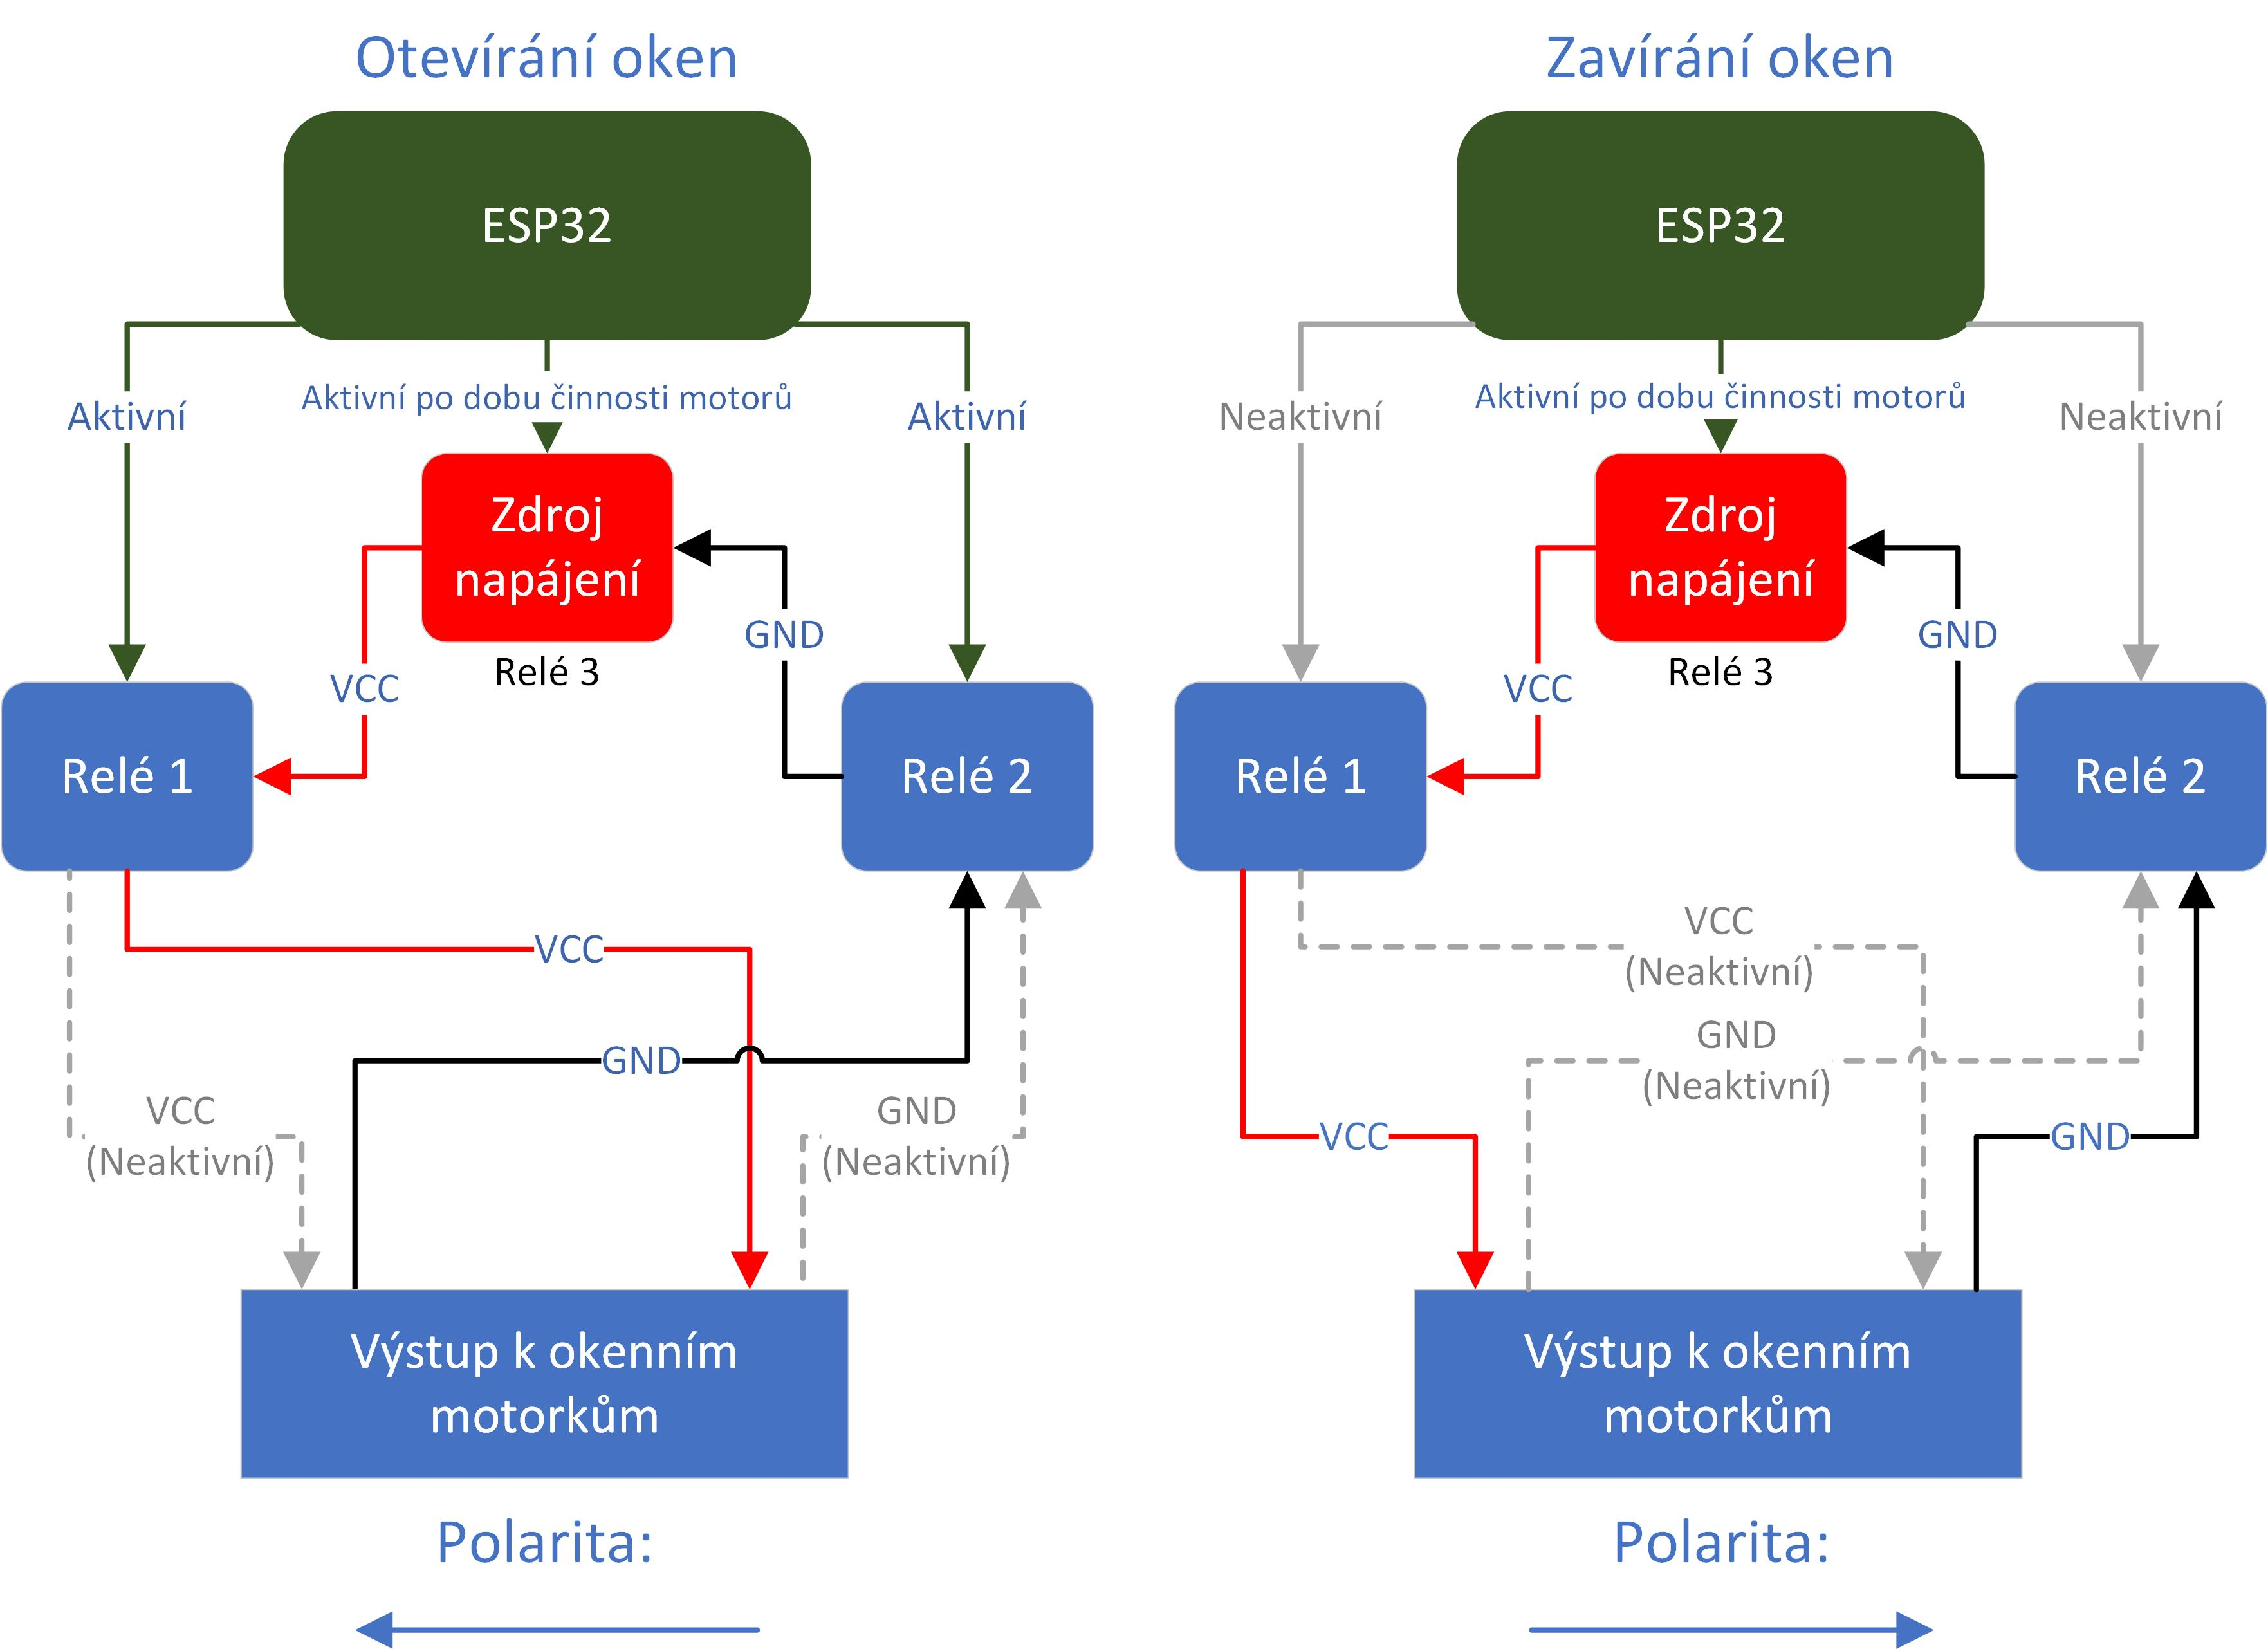
\includegraphics[width=\textwidth]{img/okna.jpg}
    \caption{Schéma funkce invertoru napětí}
    \label{fig:okna_invertory}
\end{figure} 

\begin{figure}[htbp]
 	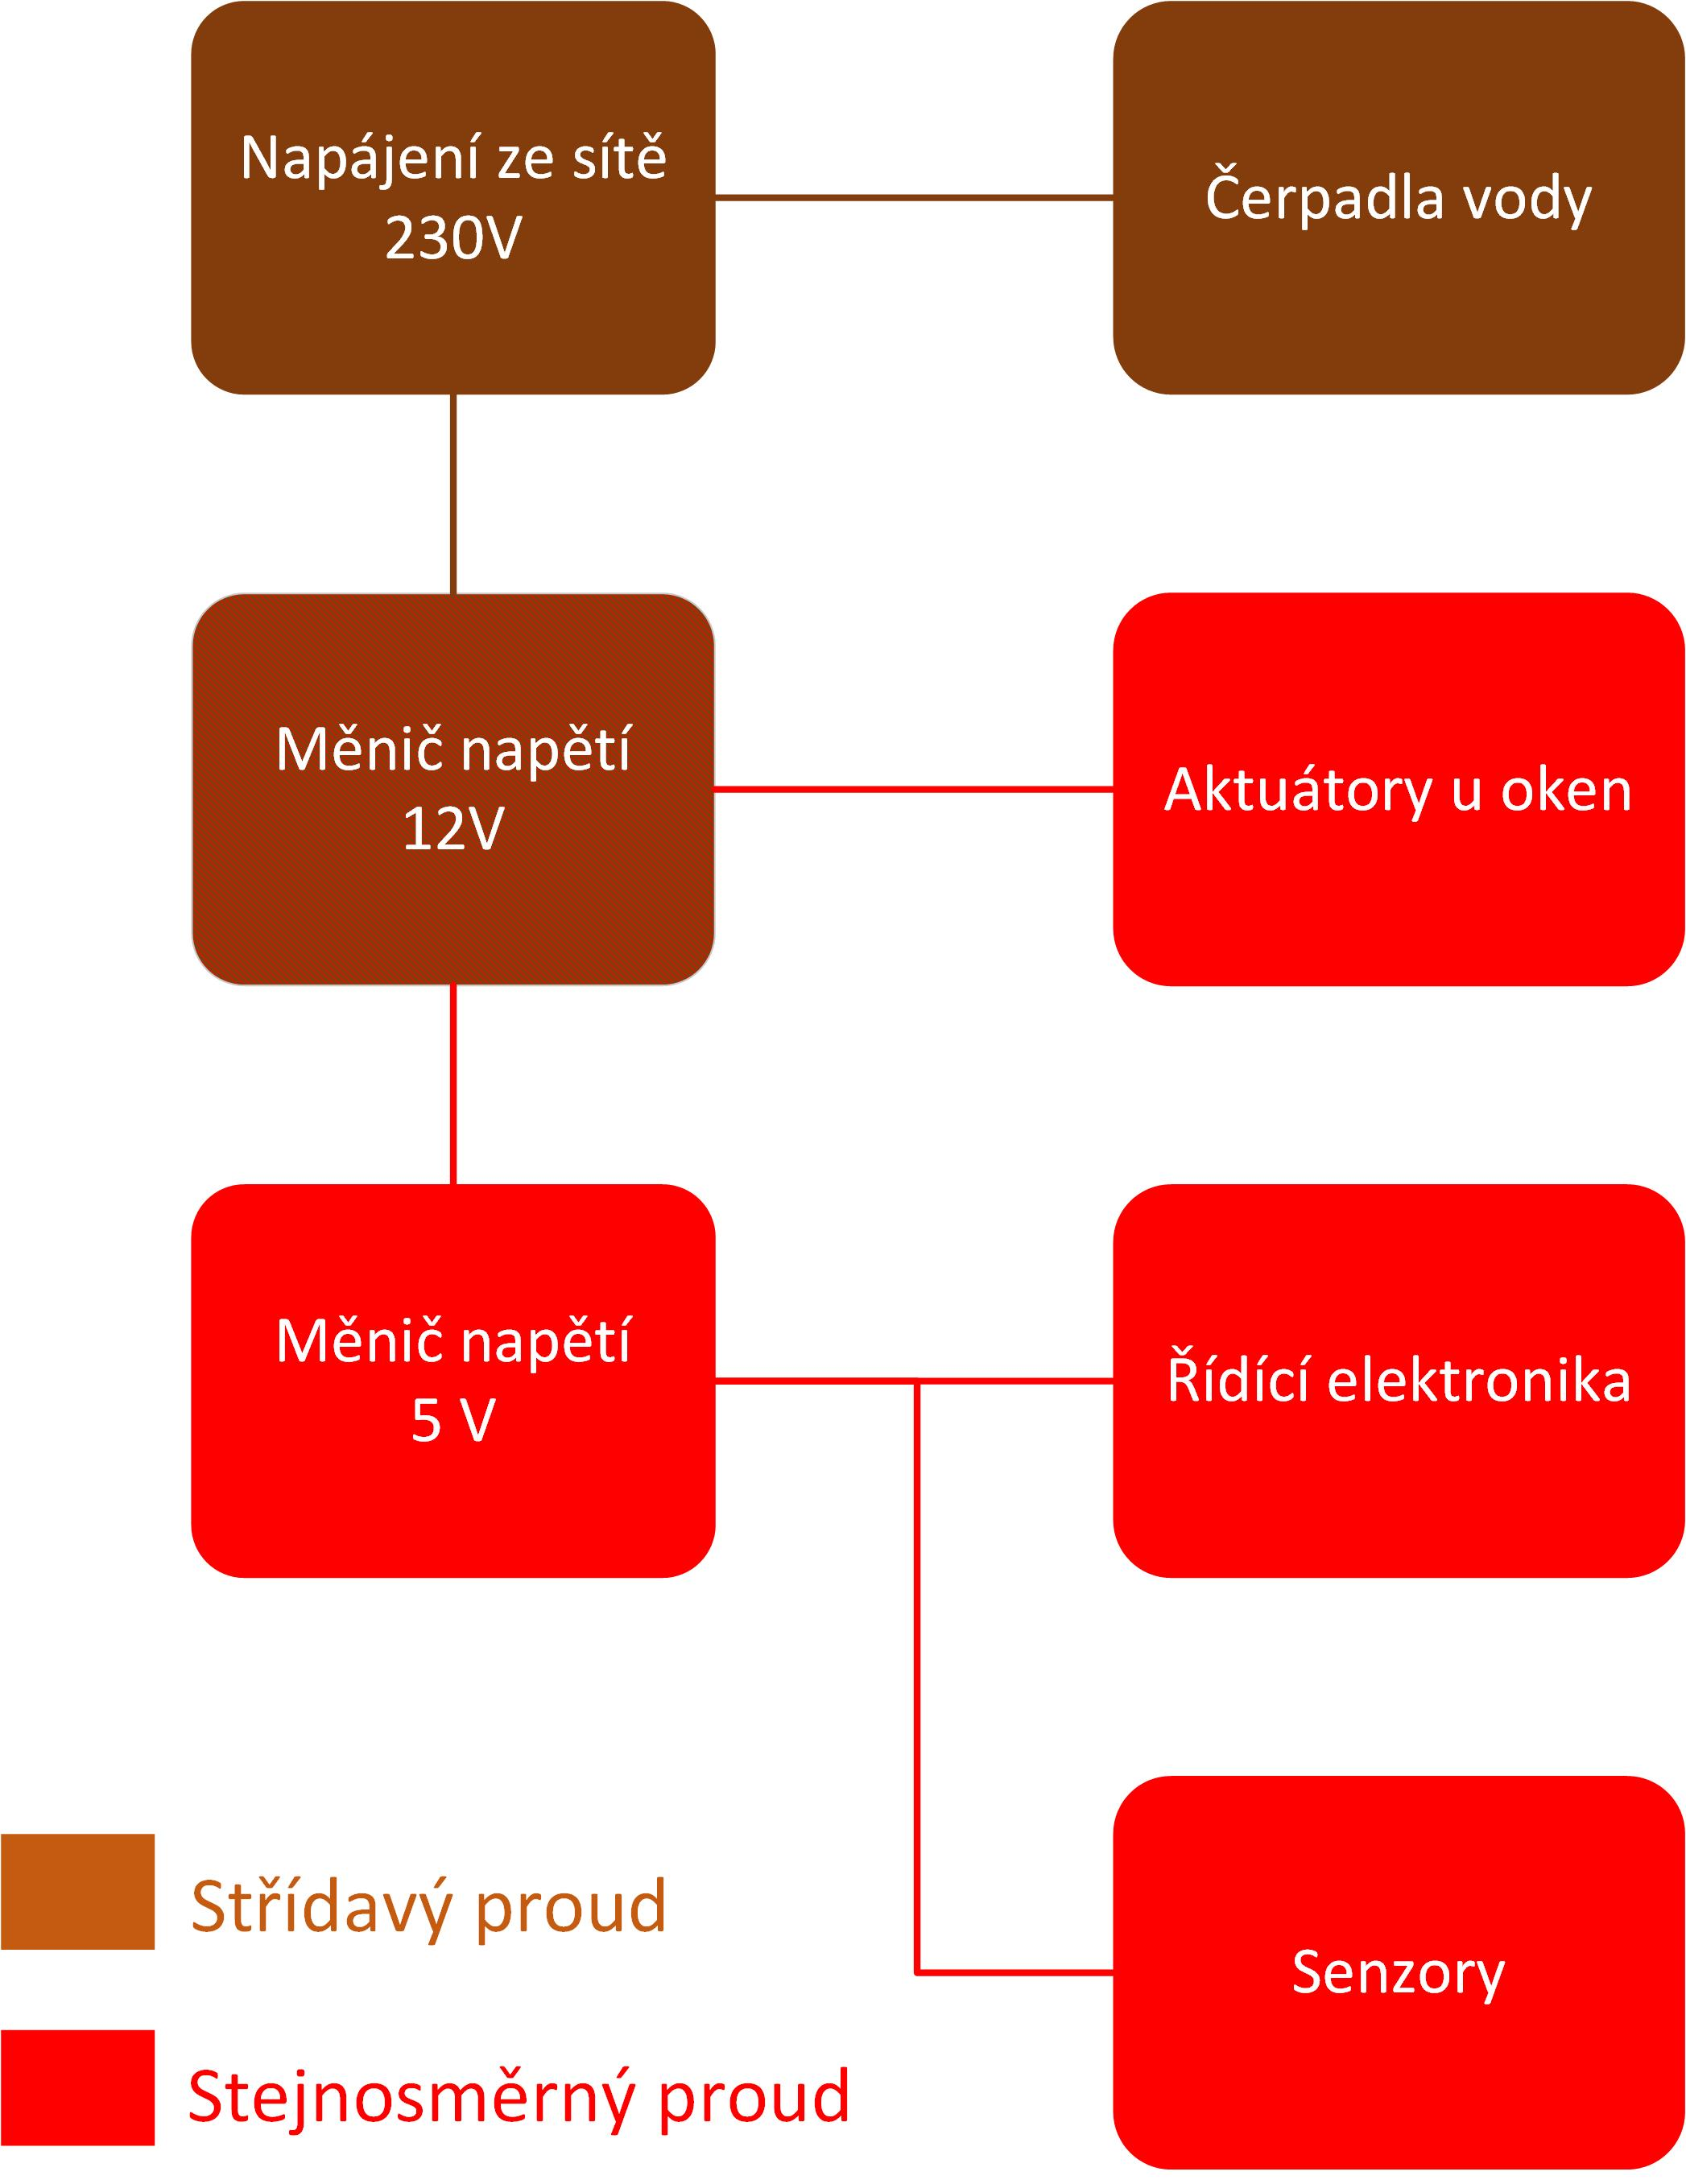
\includegraphics[width=\textwidth]{img/napajeni.jpg}
 	\caption{Schéma napájecích větví}
 	\label{fig:napajeni_vetve}
\end{figure}

\begin{figure}[htbp]
 	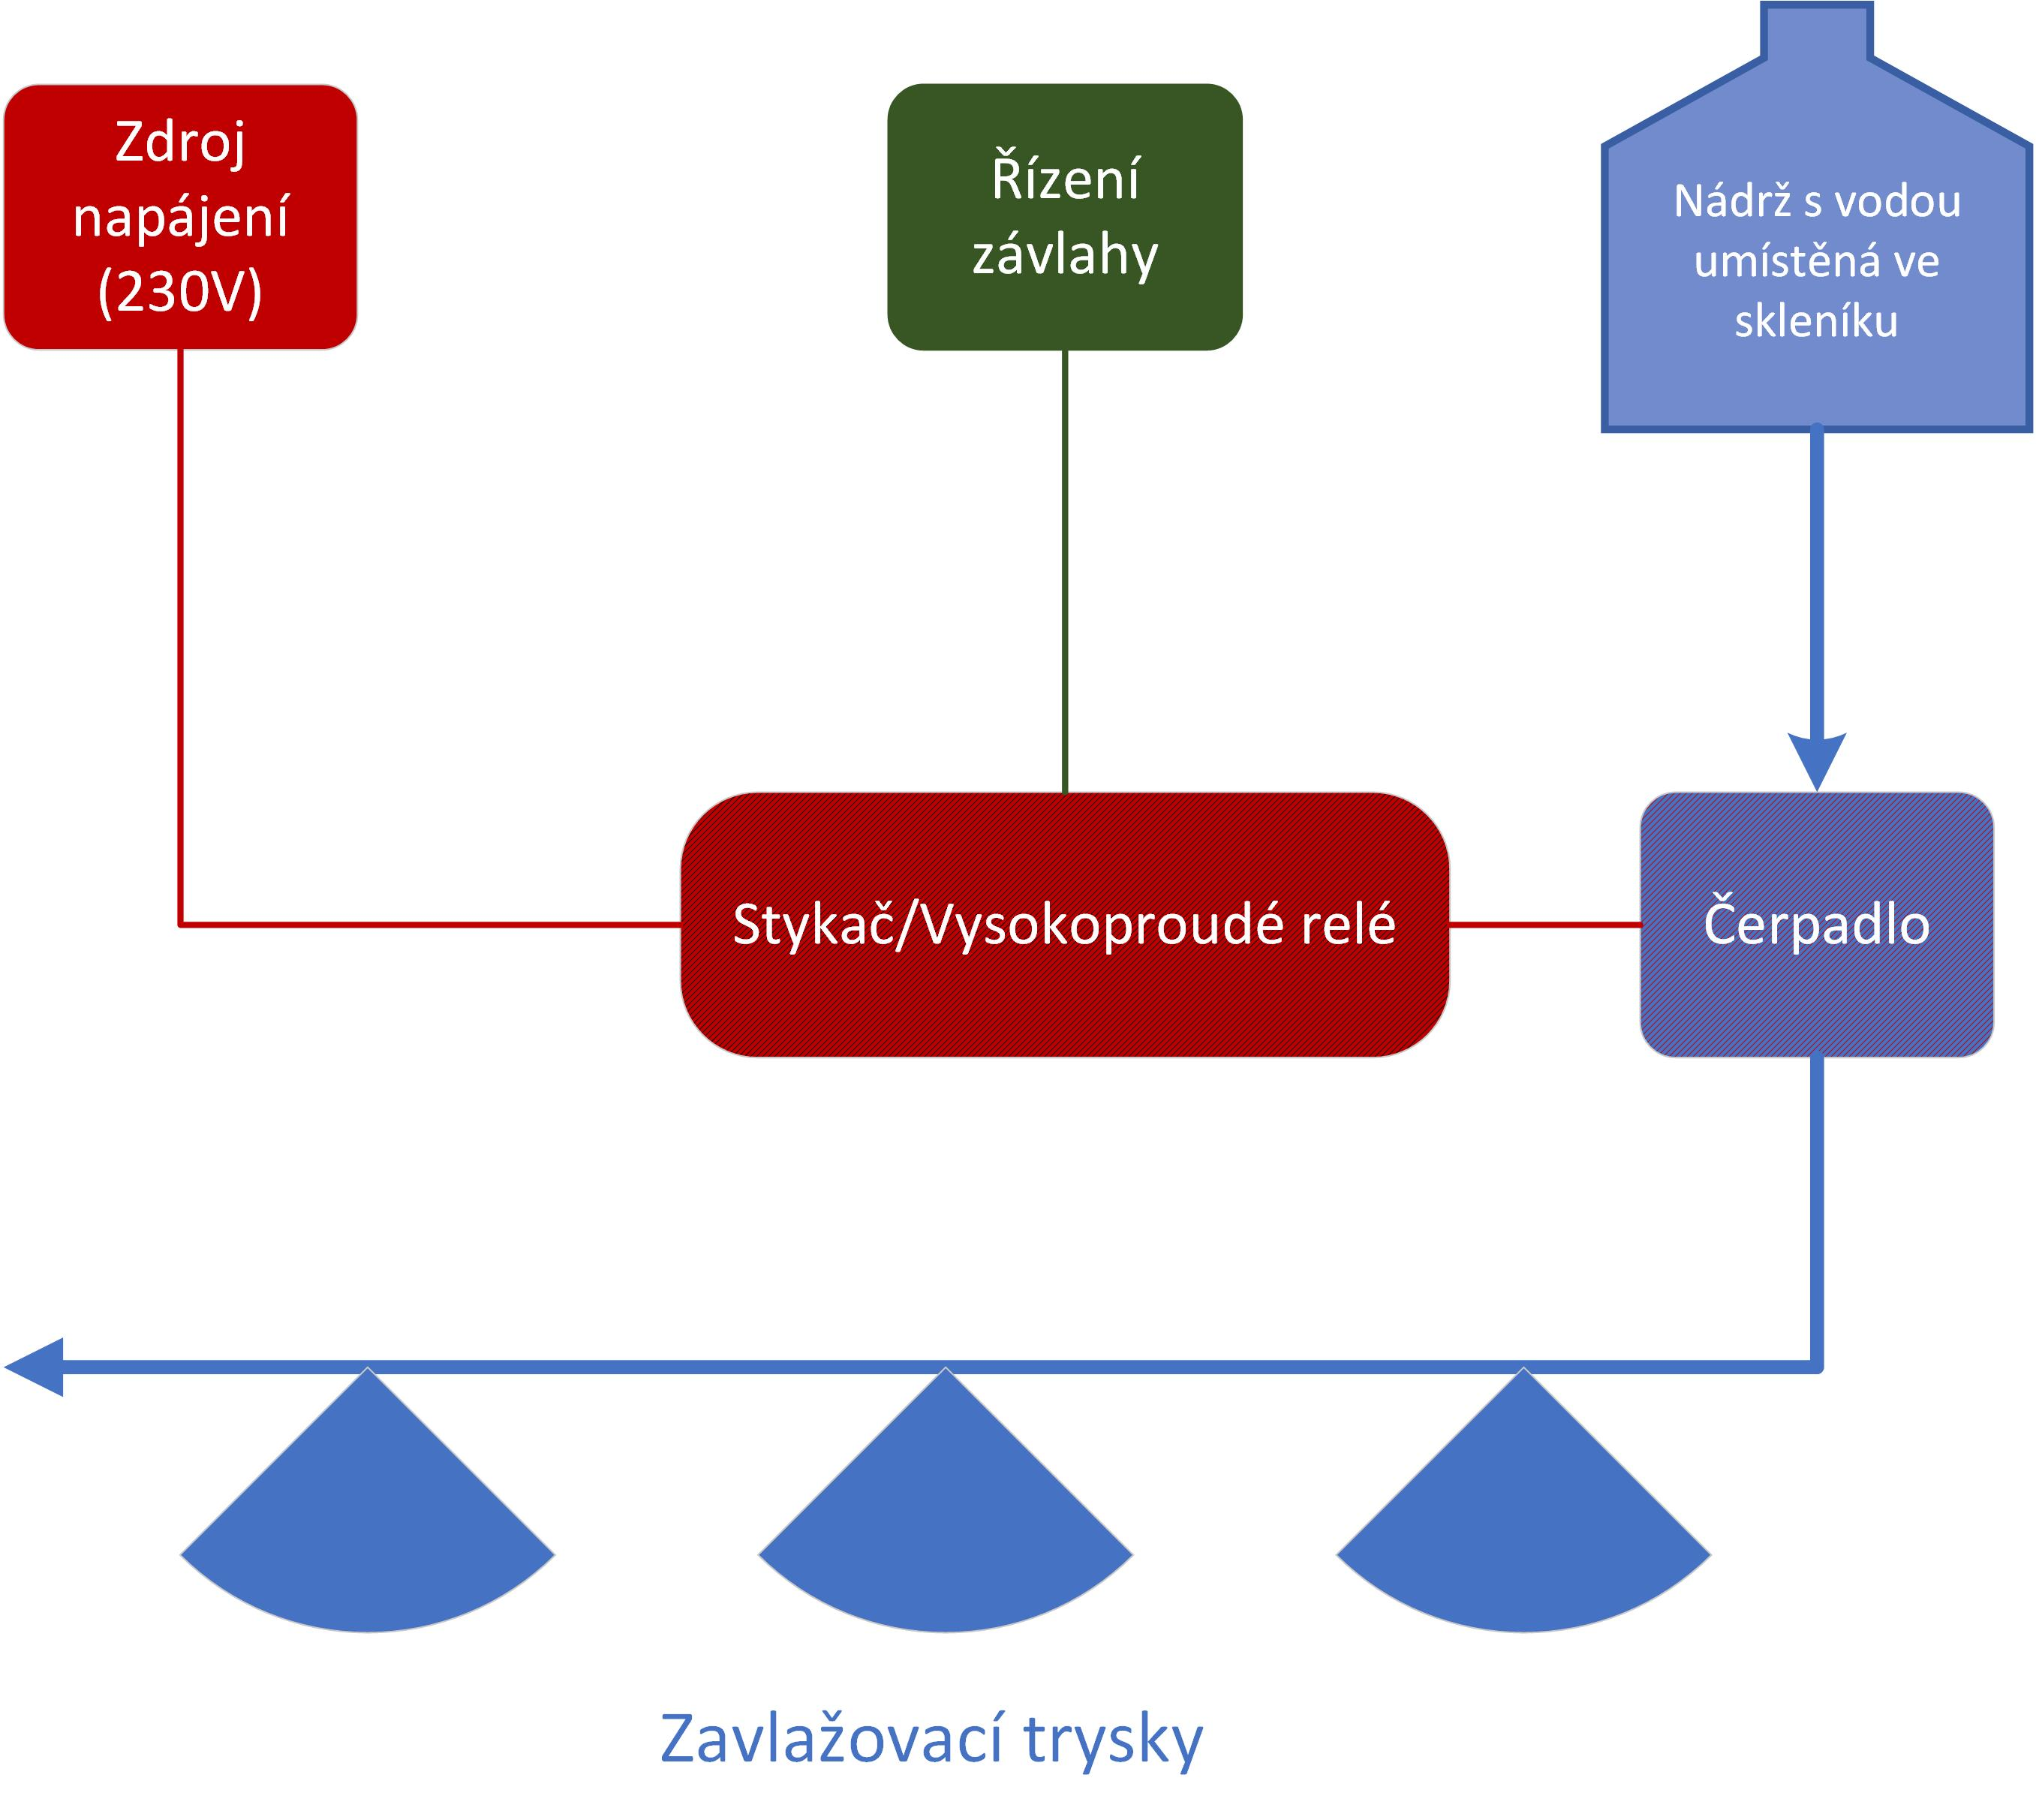
\includegraphics[width=\textwidth]{img/zavlazovani.jpg}
 	\caption{Schéma zapojení zavlažovacího systému}
 	\label{fig:zavlaha_schema} 
\end{figure}

\begin{figure}[htbp]
    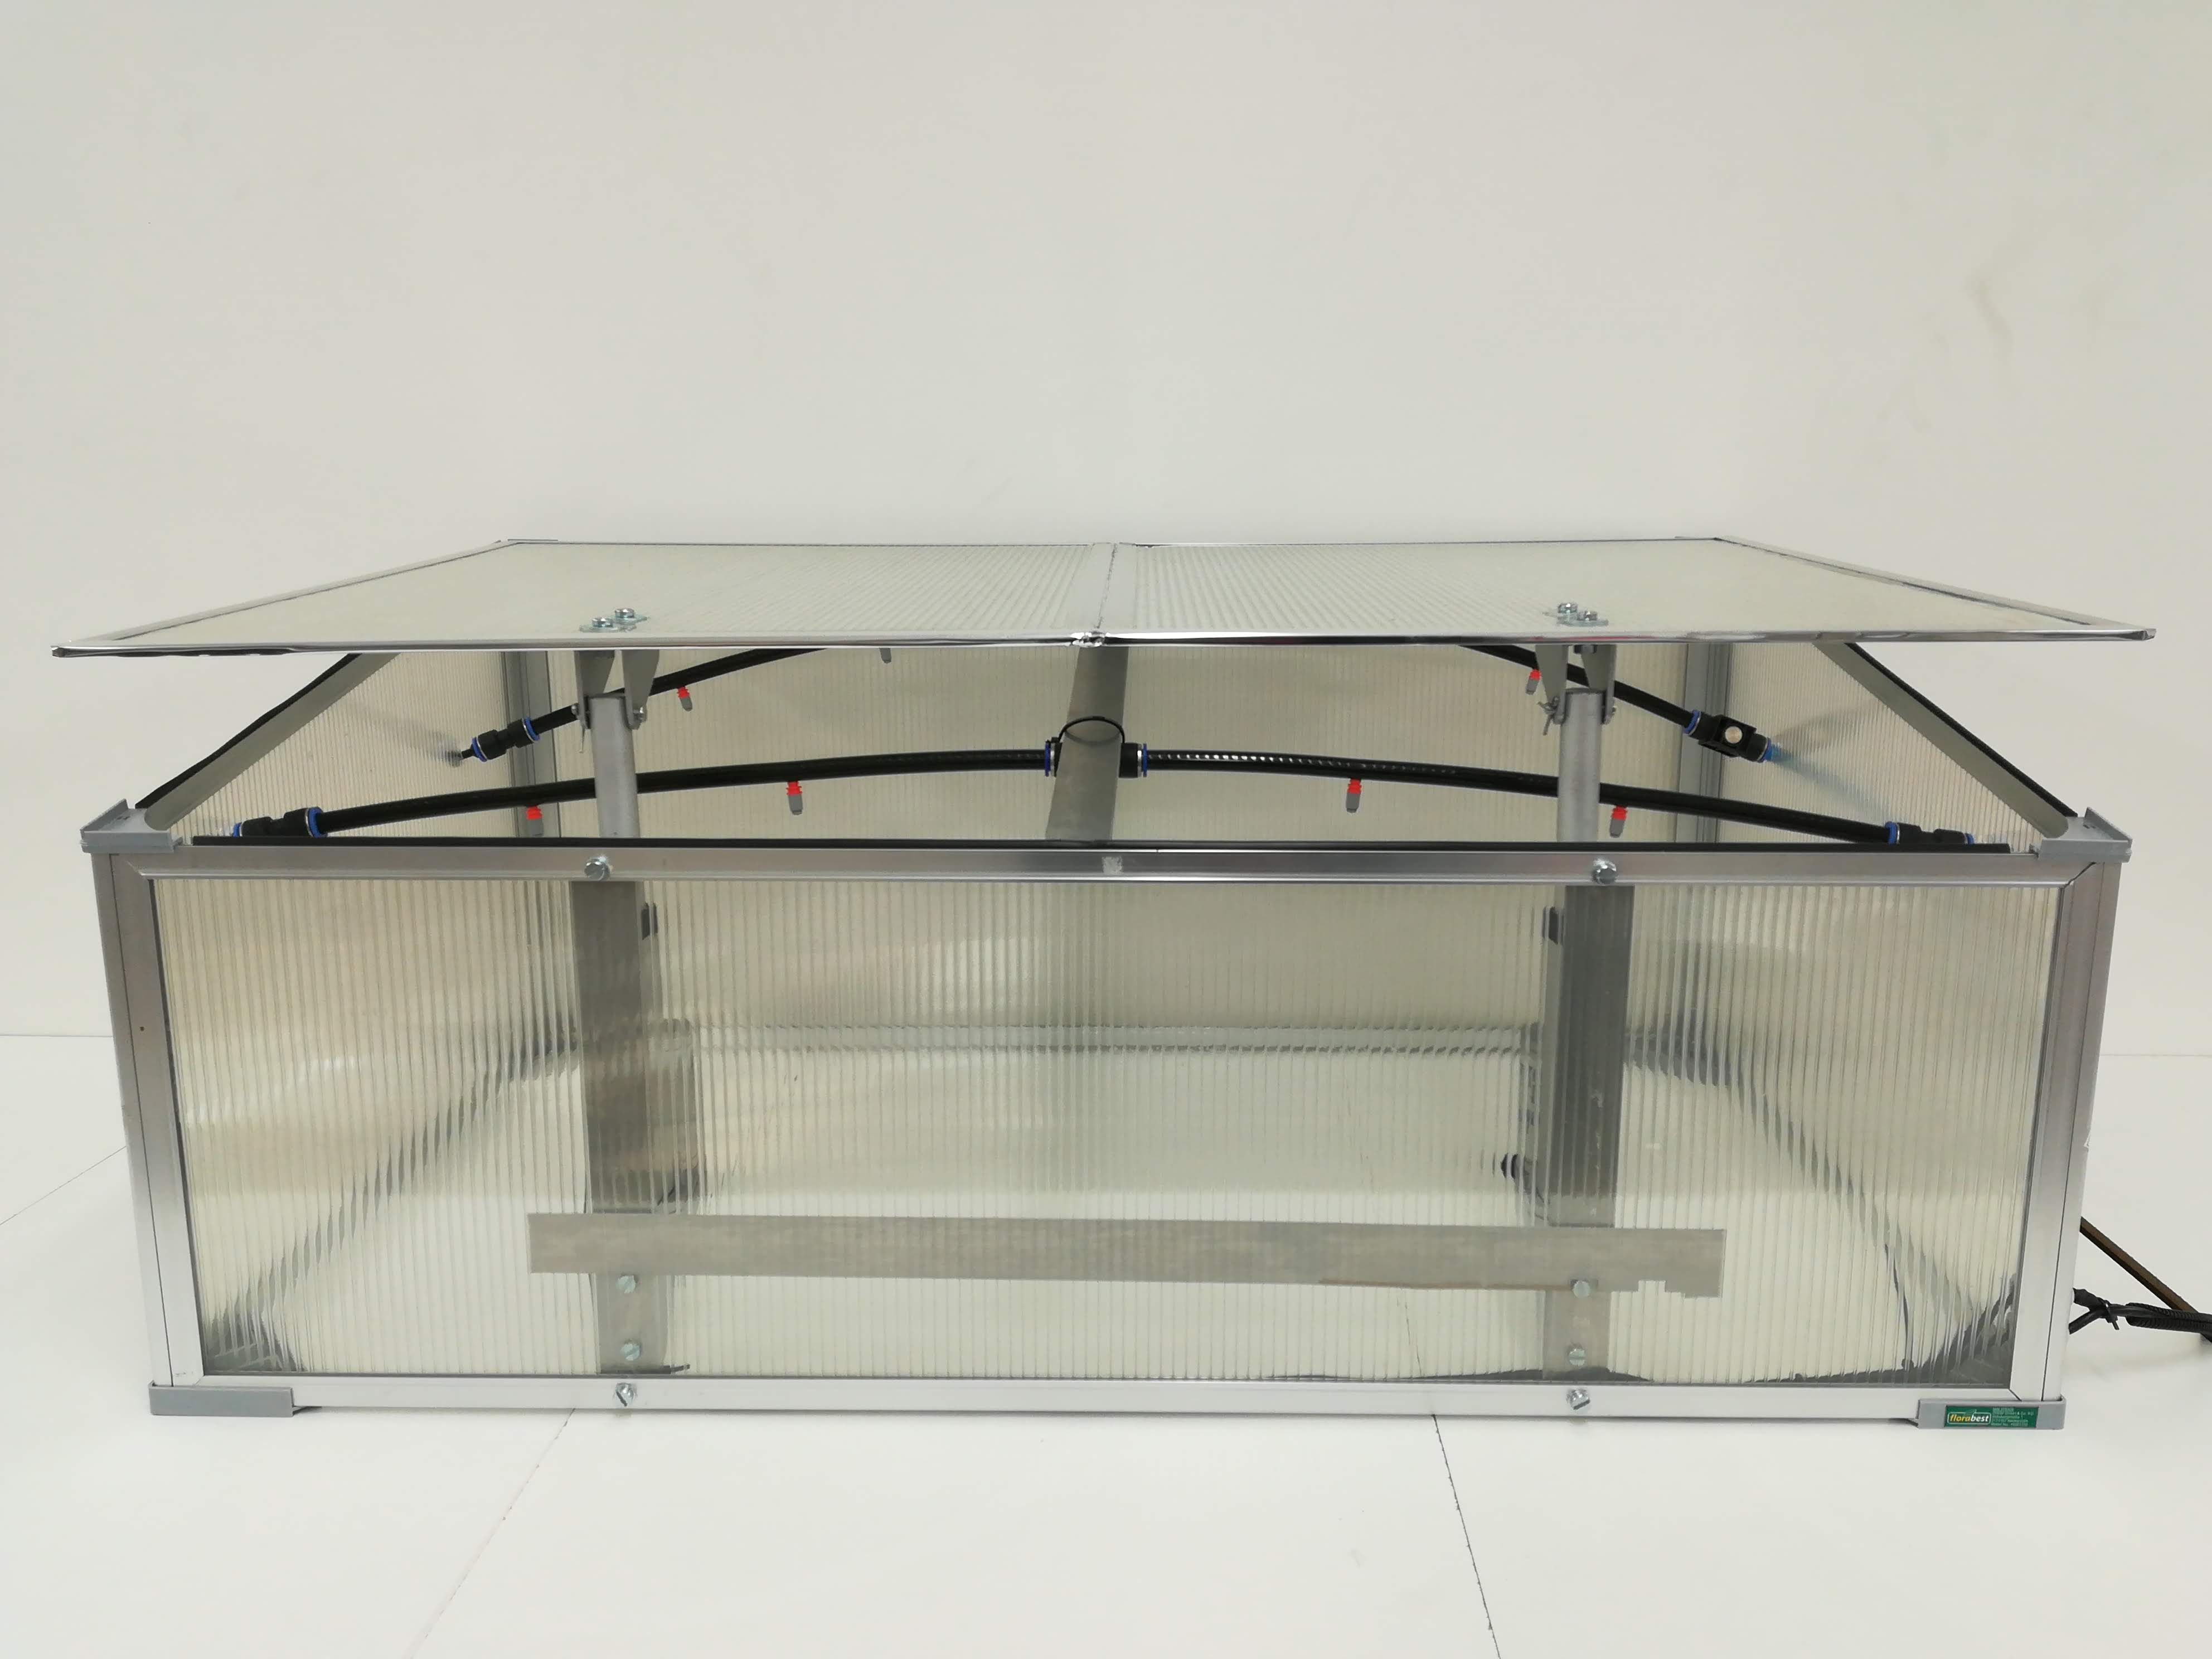
\includegraphics[width=\textwidth]{img/miniSklenik.jpg}
    \caption{Fotografie prezentační verze skleníku}
    \label{fig:miniSklenik} 
\end{figure}

\begin{figure}[htbp]
    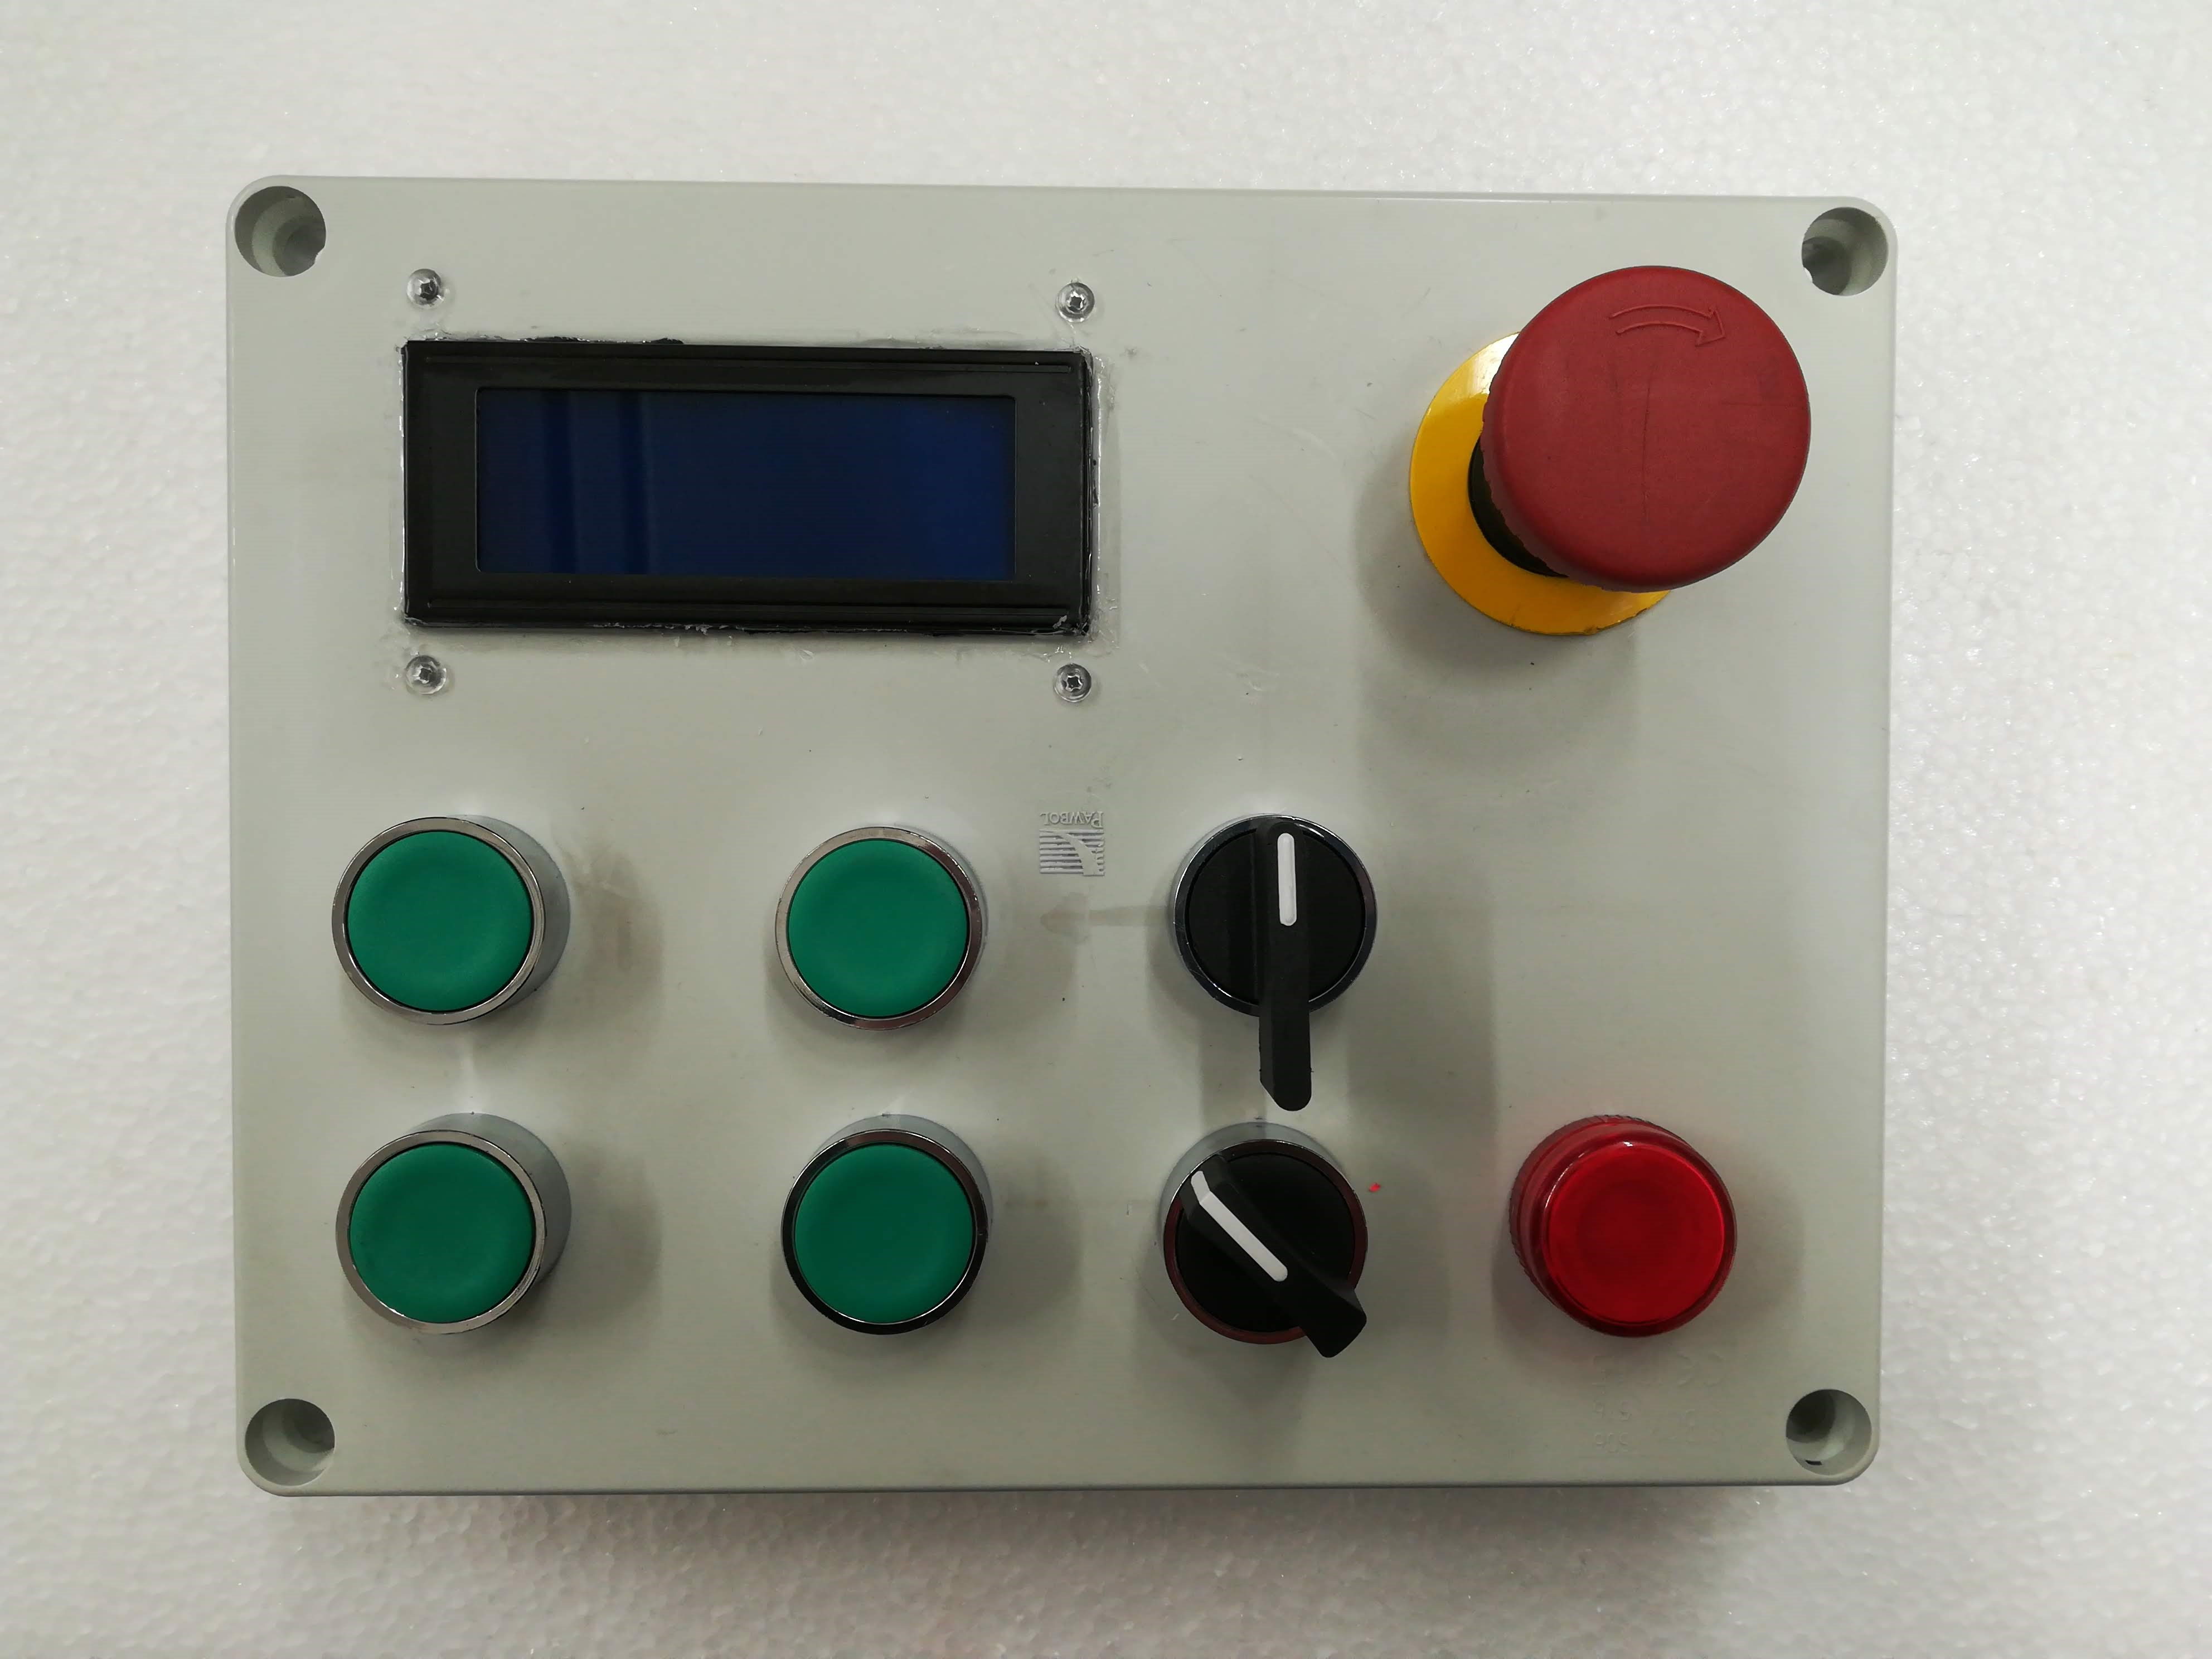
\includegraphics[width=\textwidth]{img/ridiciJednotka.jpg}
    \caption{Fotografie předního panelu řídící jednotky}
    \label{fig:panel} 
\end{figure}

\begin{figure}[htbp]
    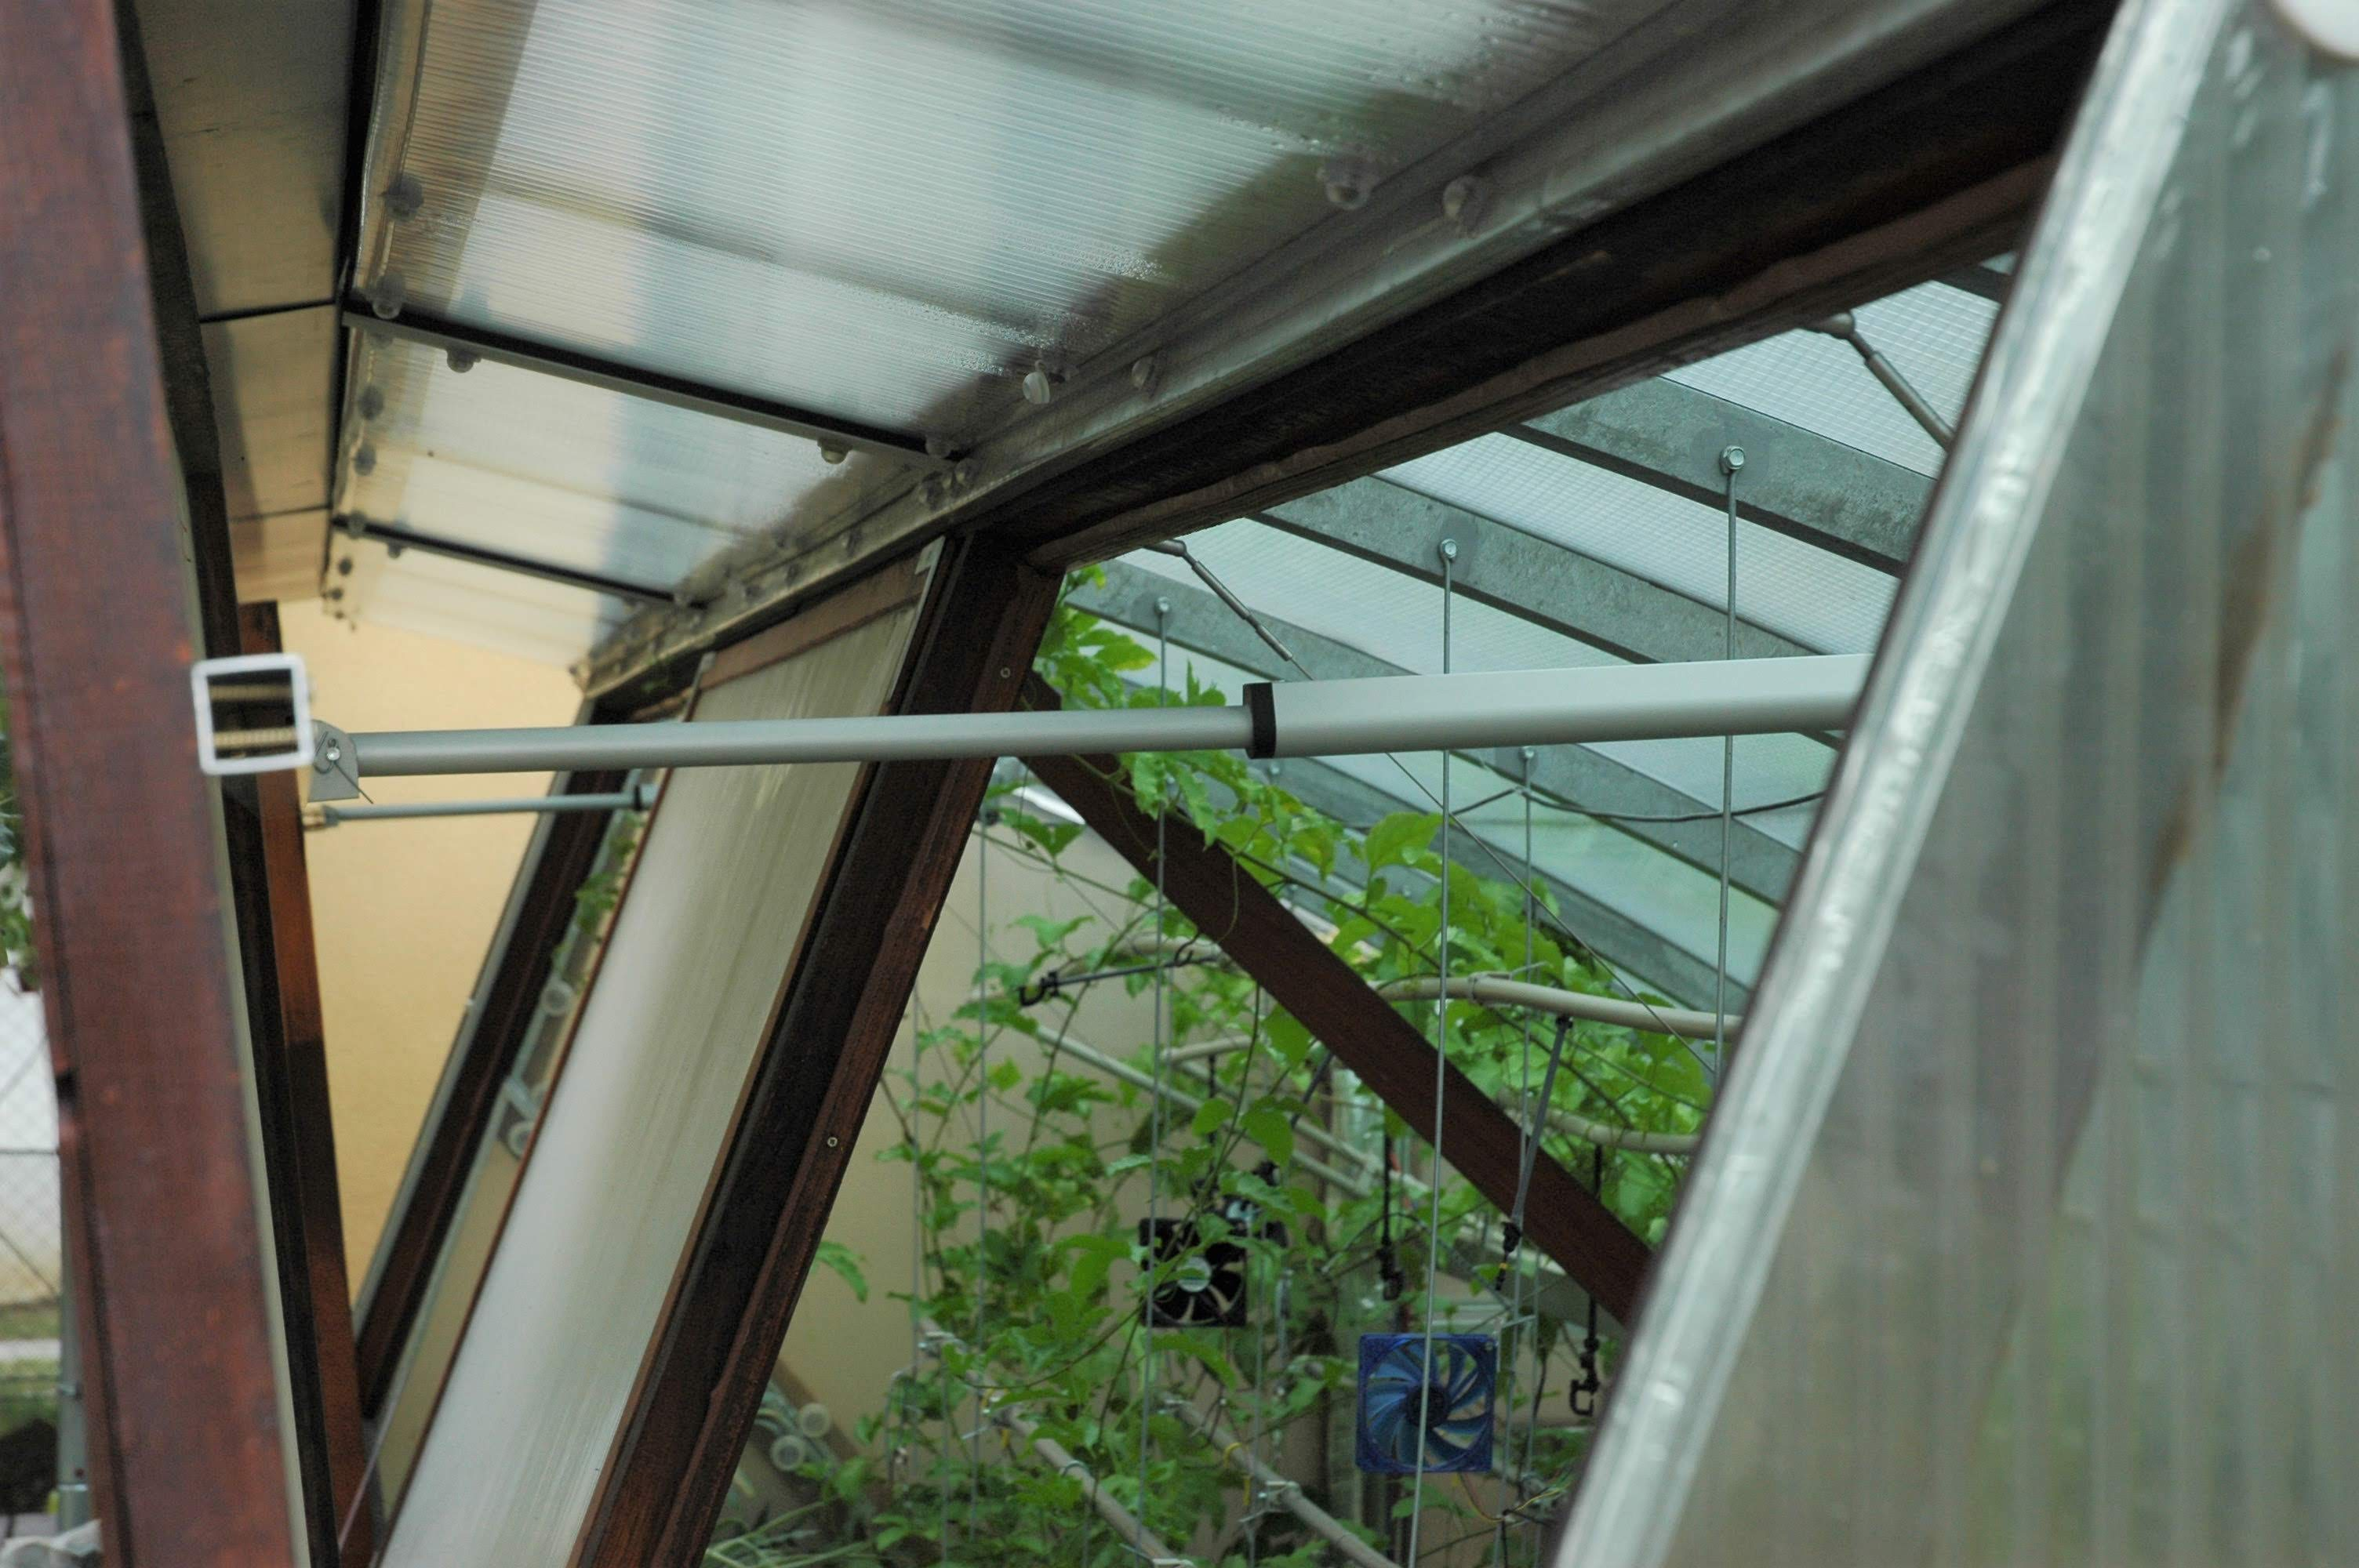
\includegraphics[width=\textwidth]{img/VS_1.jpg}
    \caption{Fotografie velkého skleníku}
    \label{fig:VS1} 
\end{figure}

\begin{figure}[htbp]
    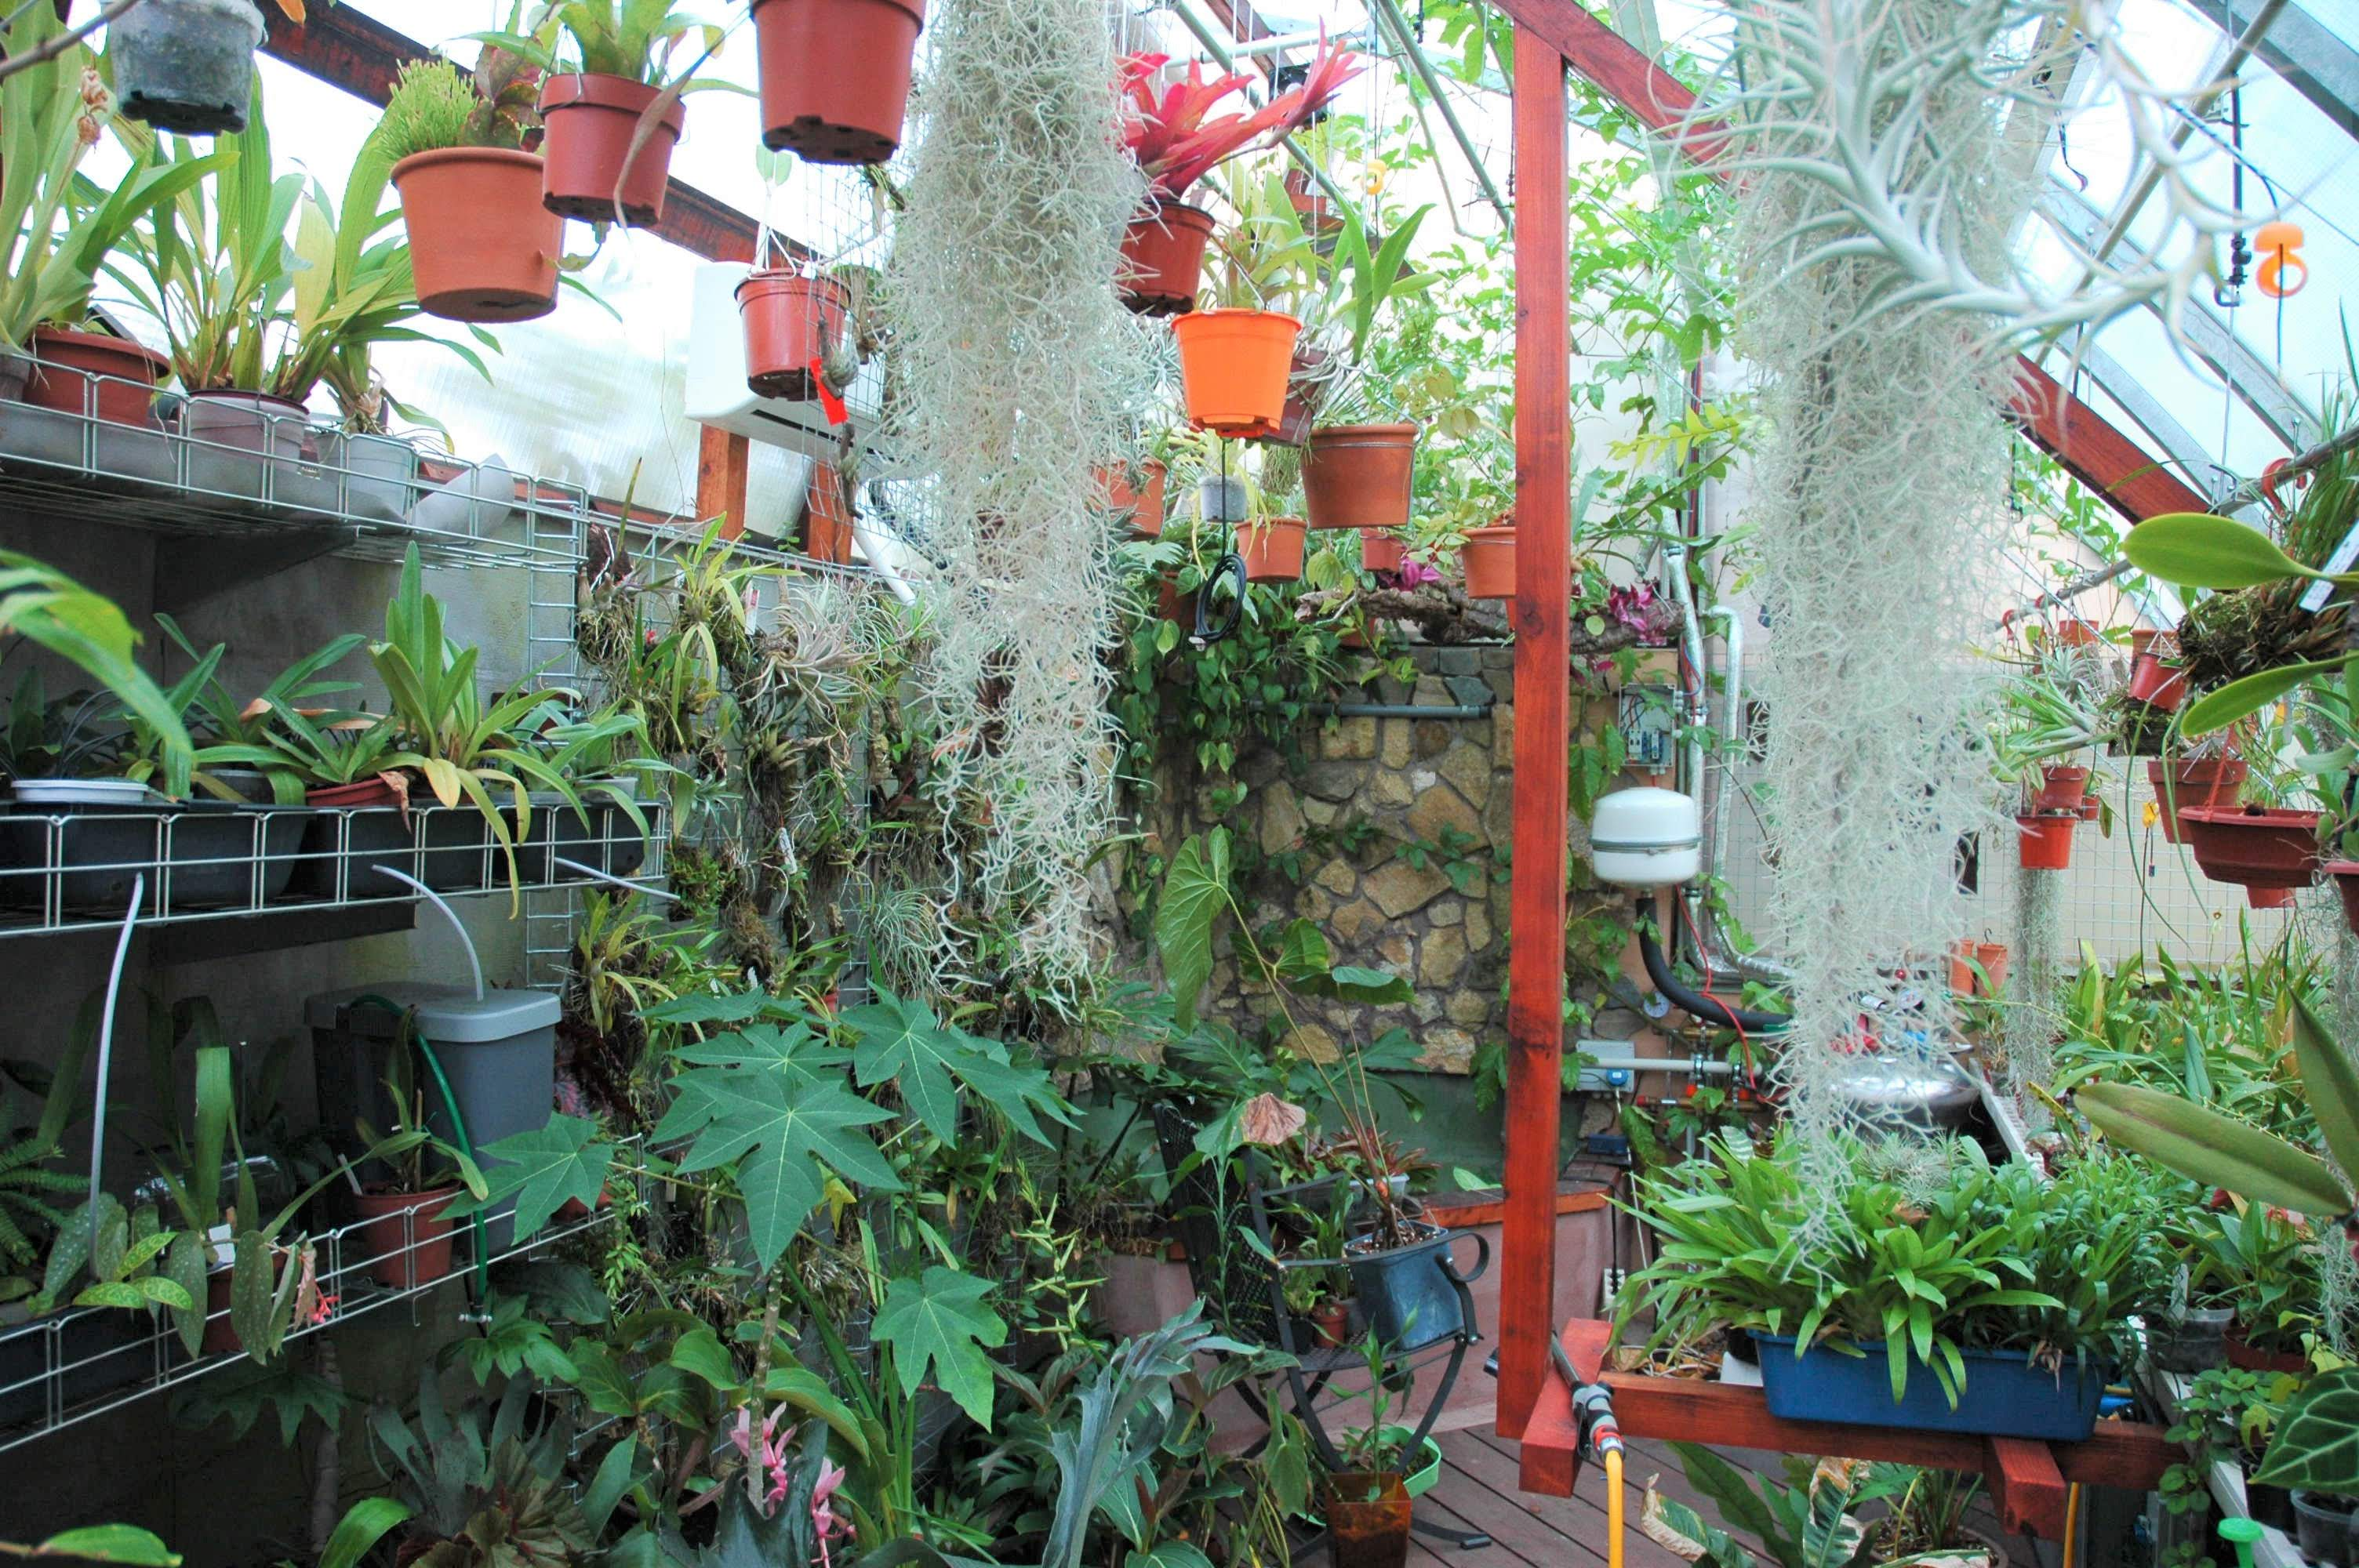
\includegraphics[width=\textwidth]{img/VS_2.jpg}
    \caption{Fotografie velkého skleníku}
    \label{fig:VS2} 
\end{figure}

\begin{figure}[htbp]
    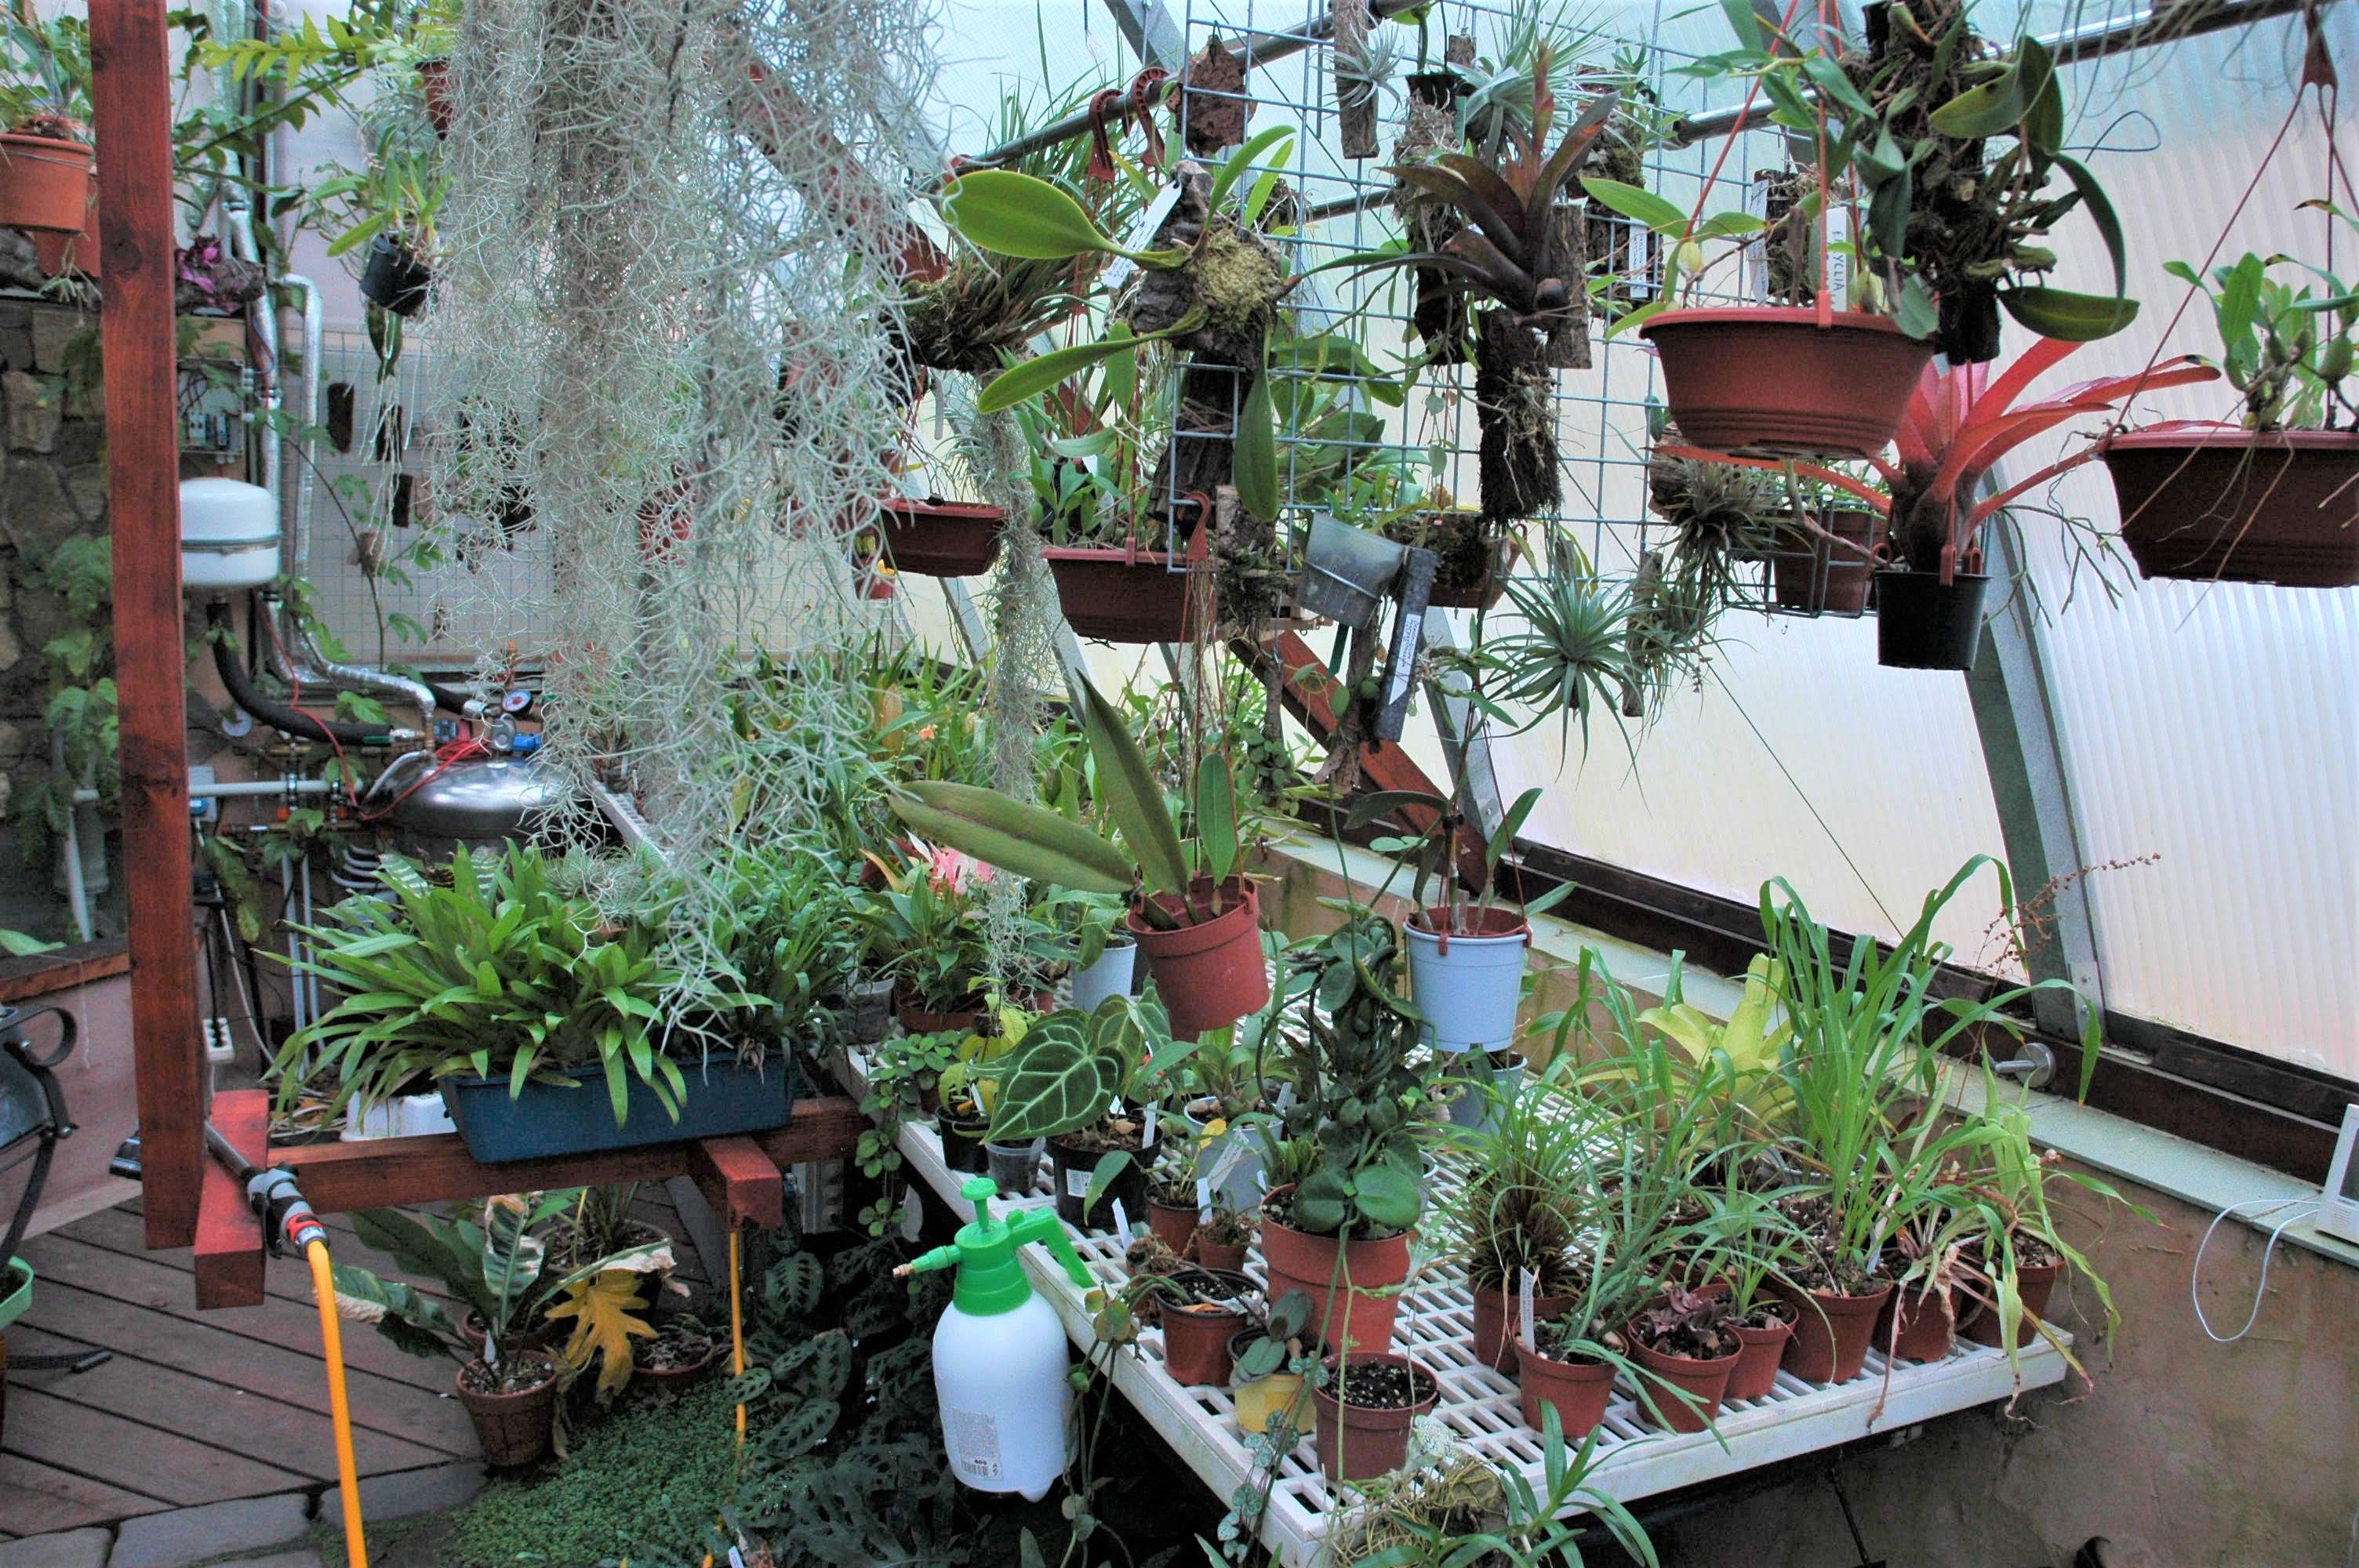
\includegraphics[width=\textwidth]{img/VS_3.jpg}
    \caption{Fotografie velkého skleníku}
    \label{fig:VS3} 
\end{figure}

\begin{figure}[htbp]
    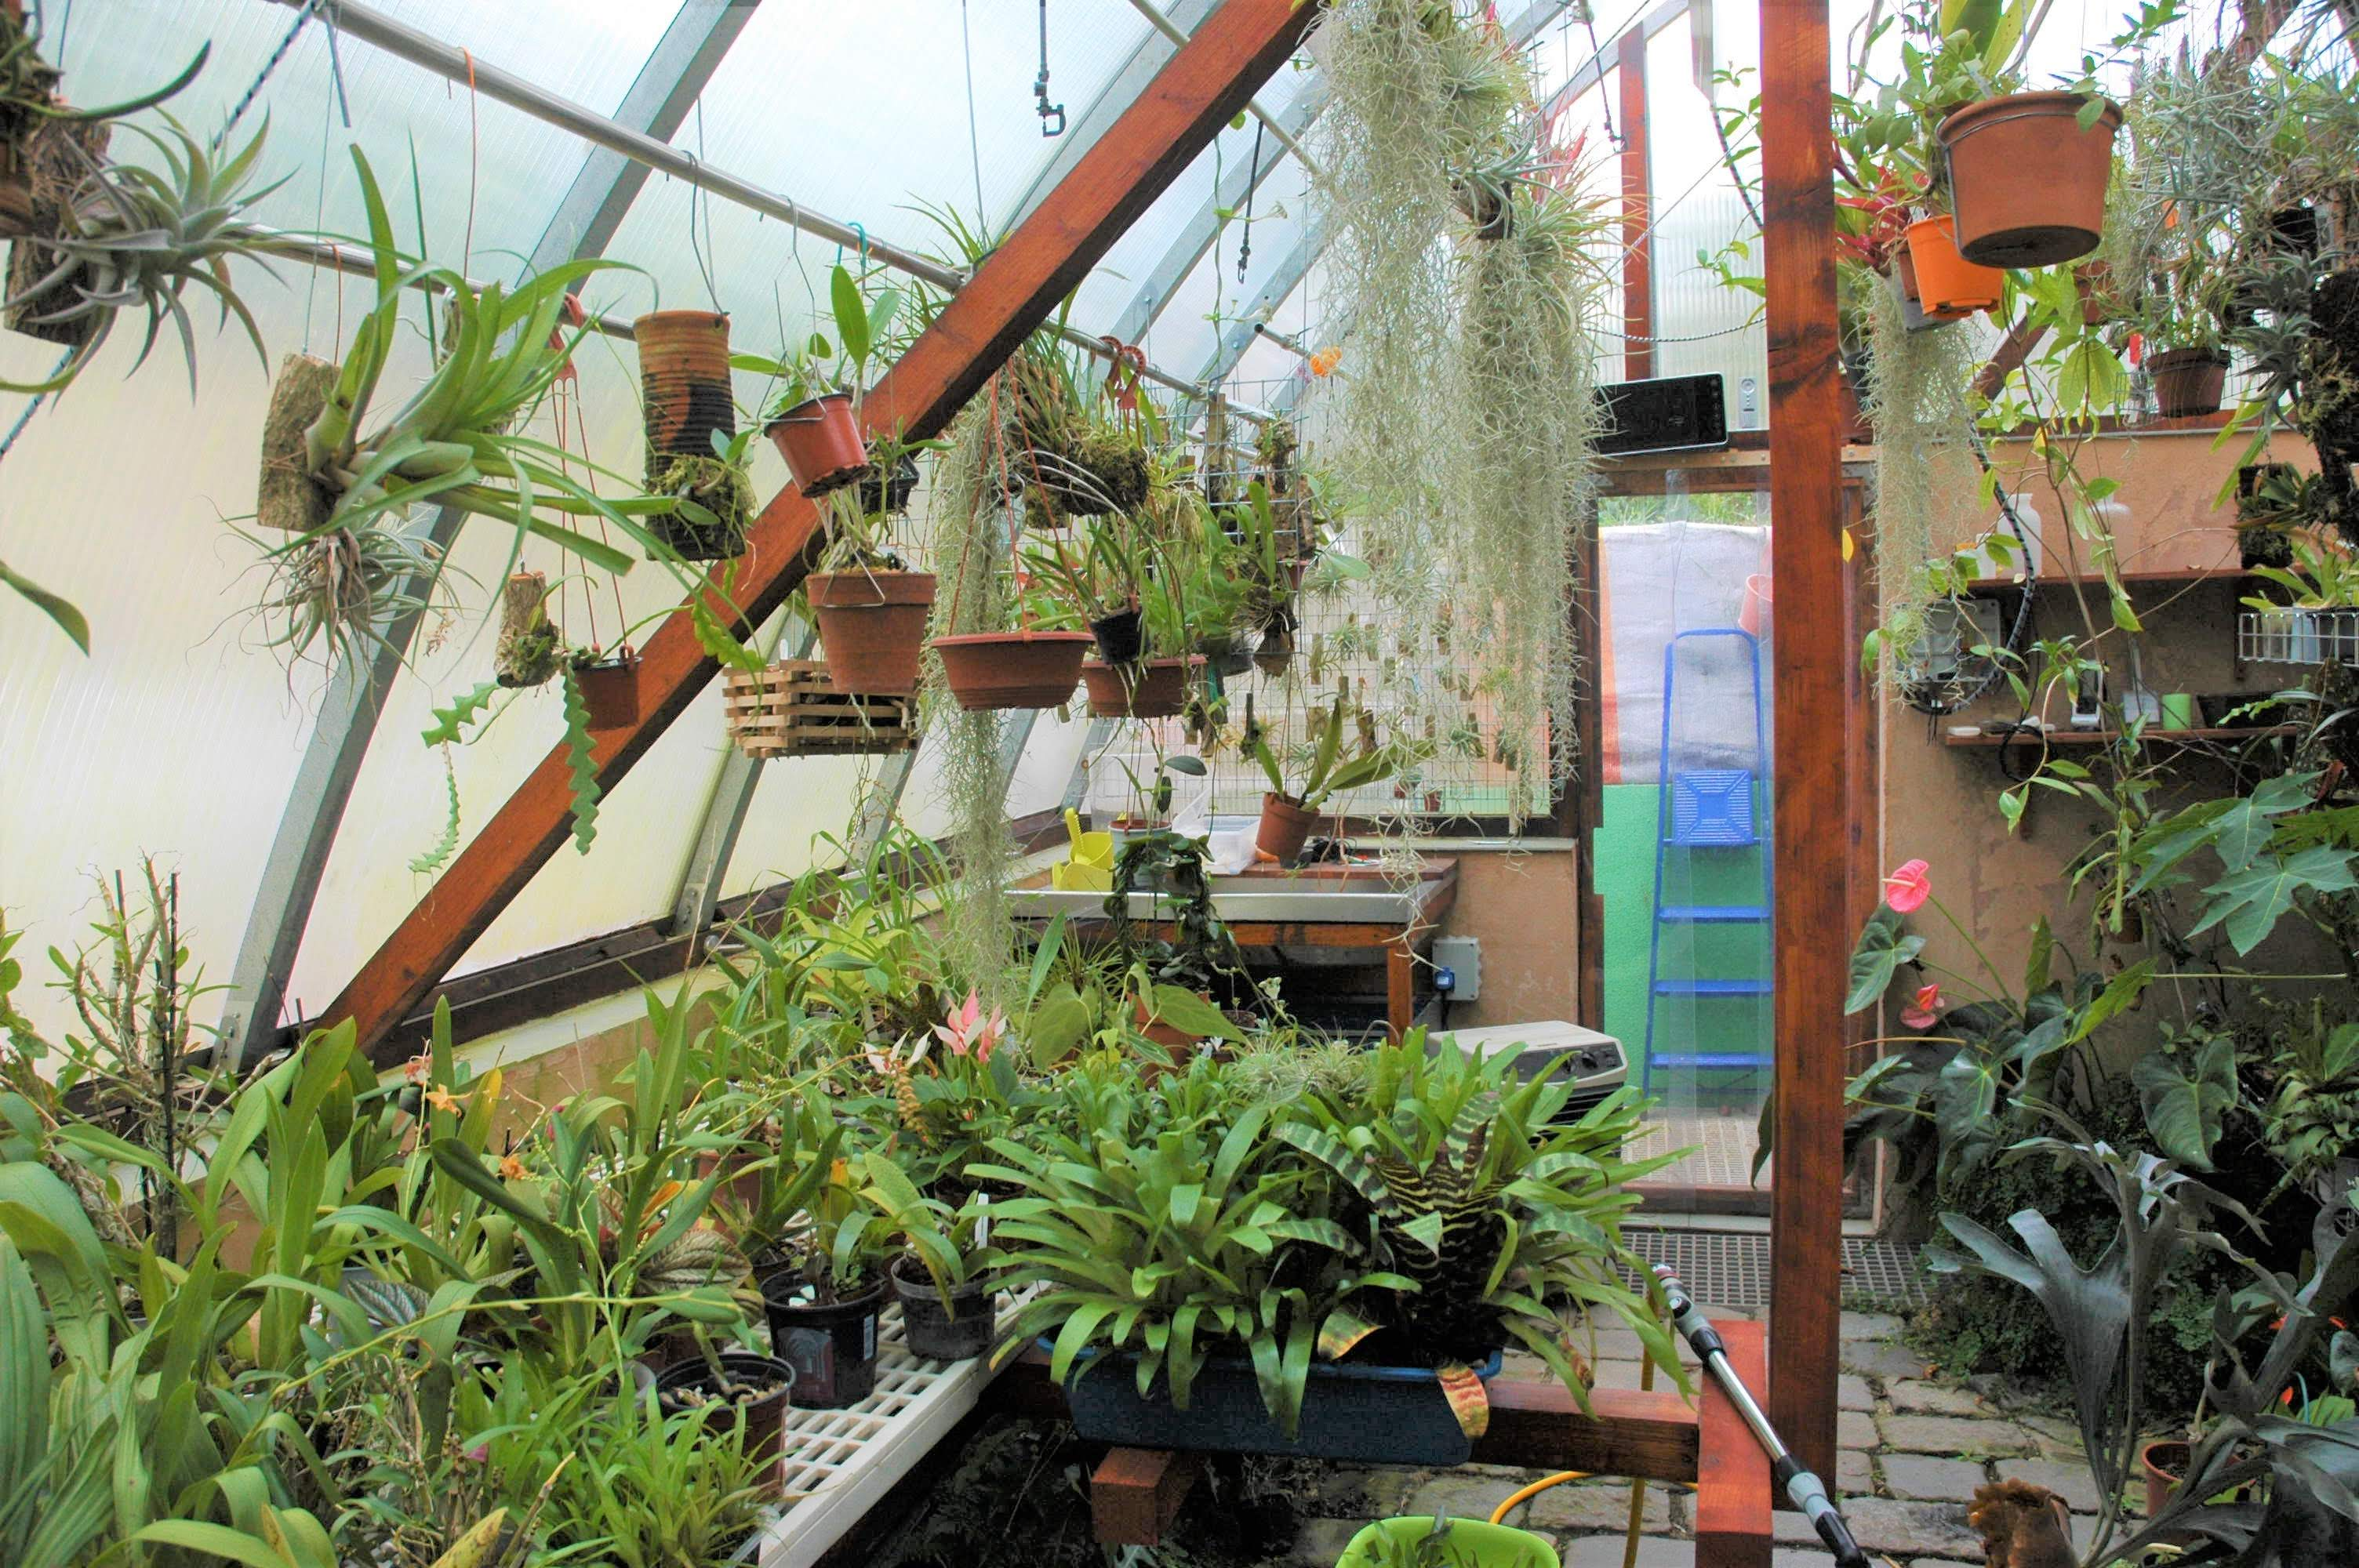
\includegraphics[width=\textwidth]{img/VS_4.jpg}
    \caption{Fotografie velkého skleníku}
    \label{fig:VS4} 
\end{figure}

\begin{figure}[htbp]
    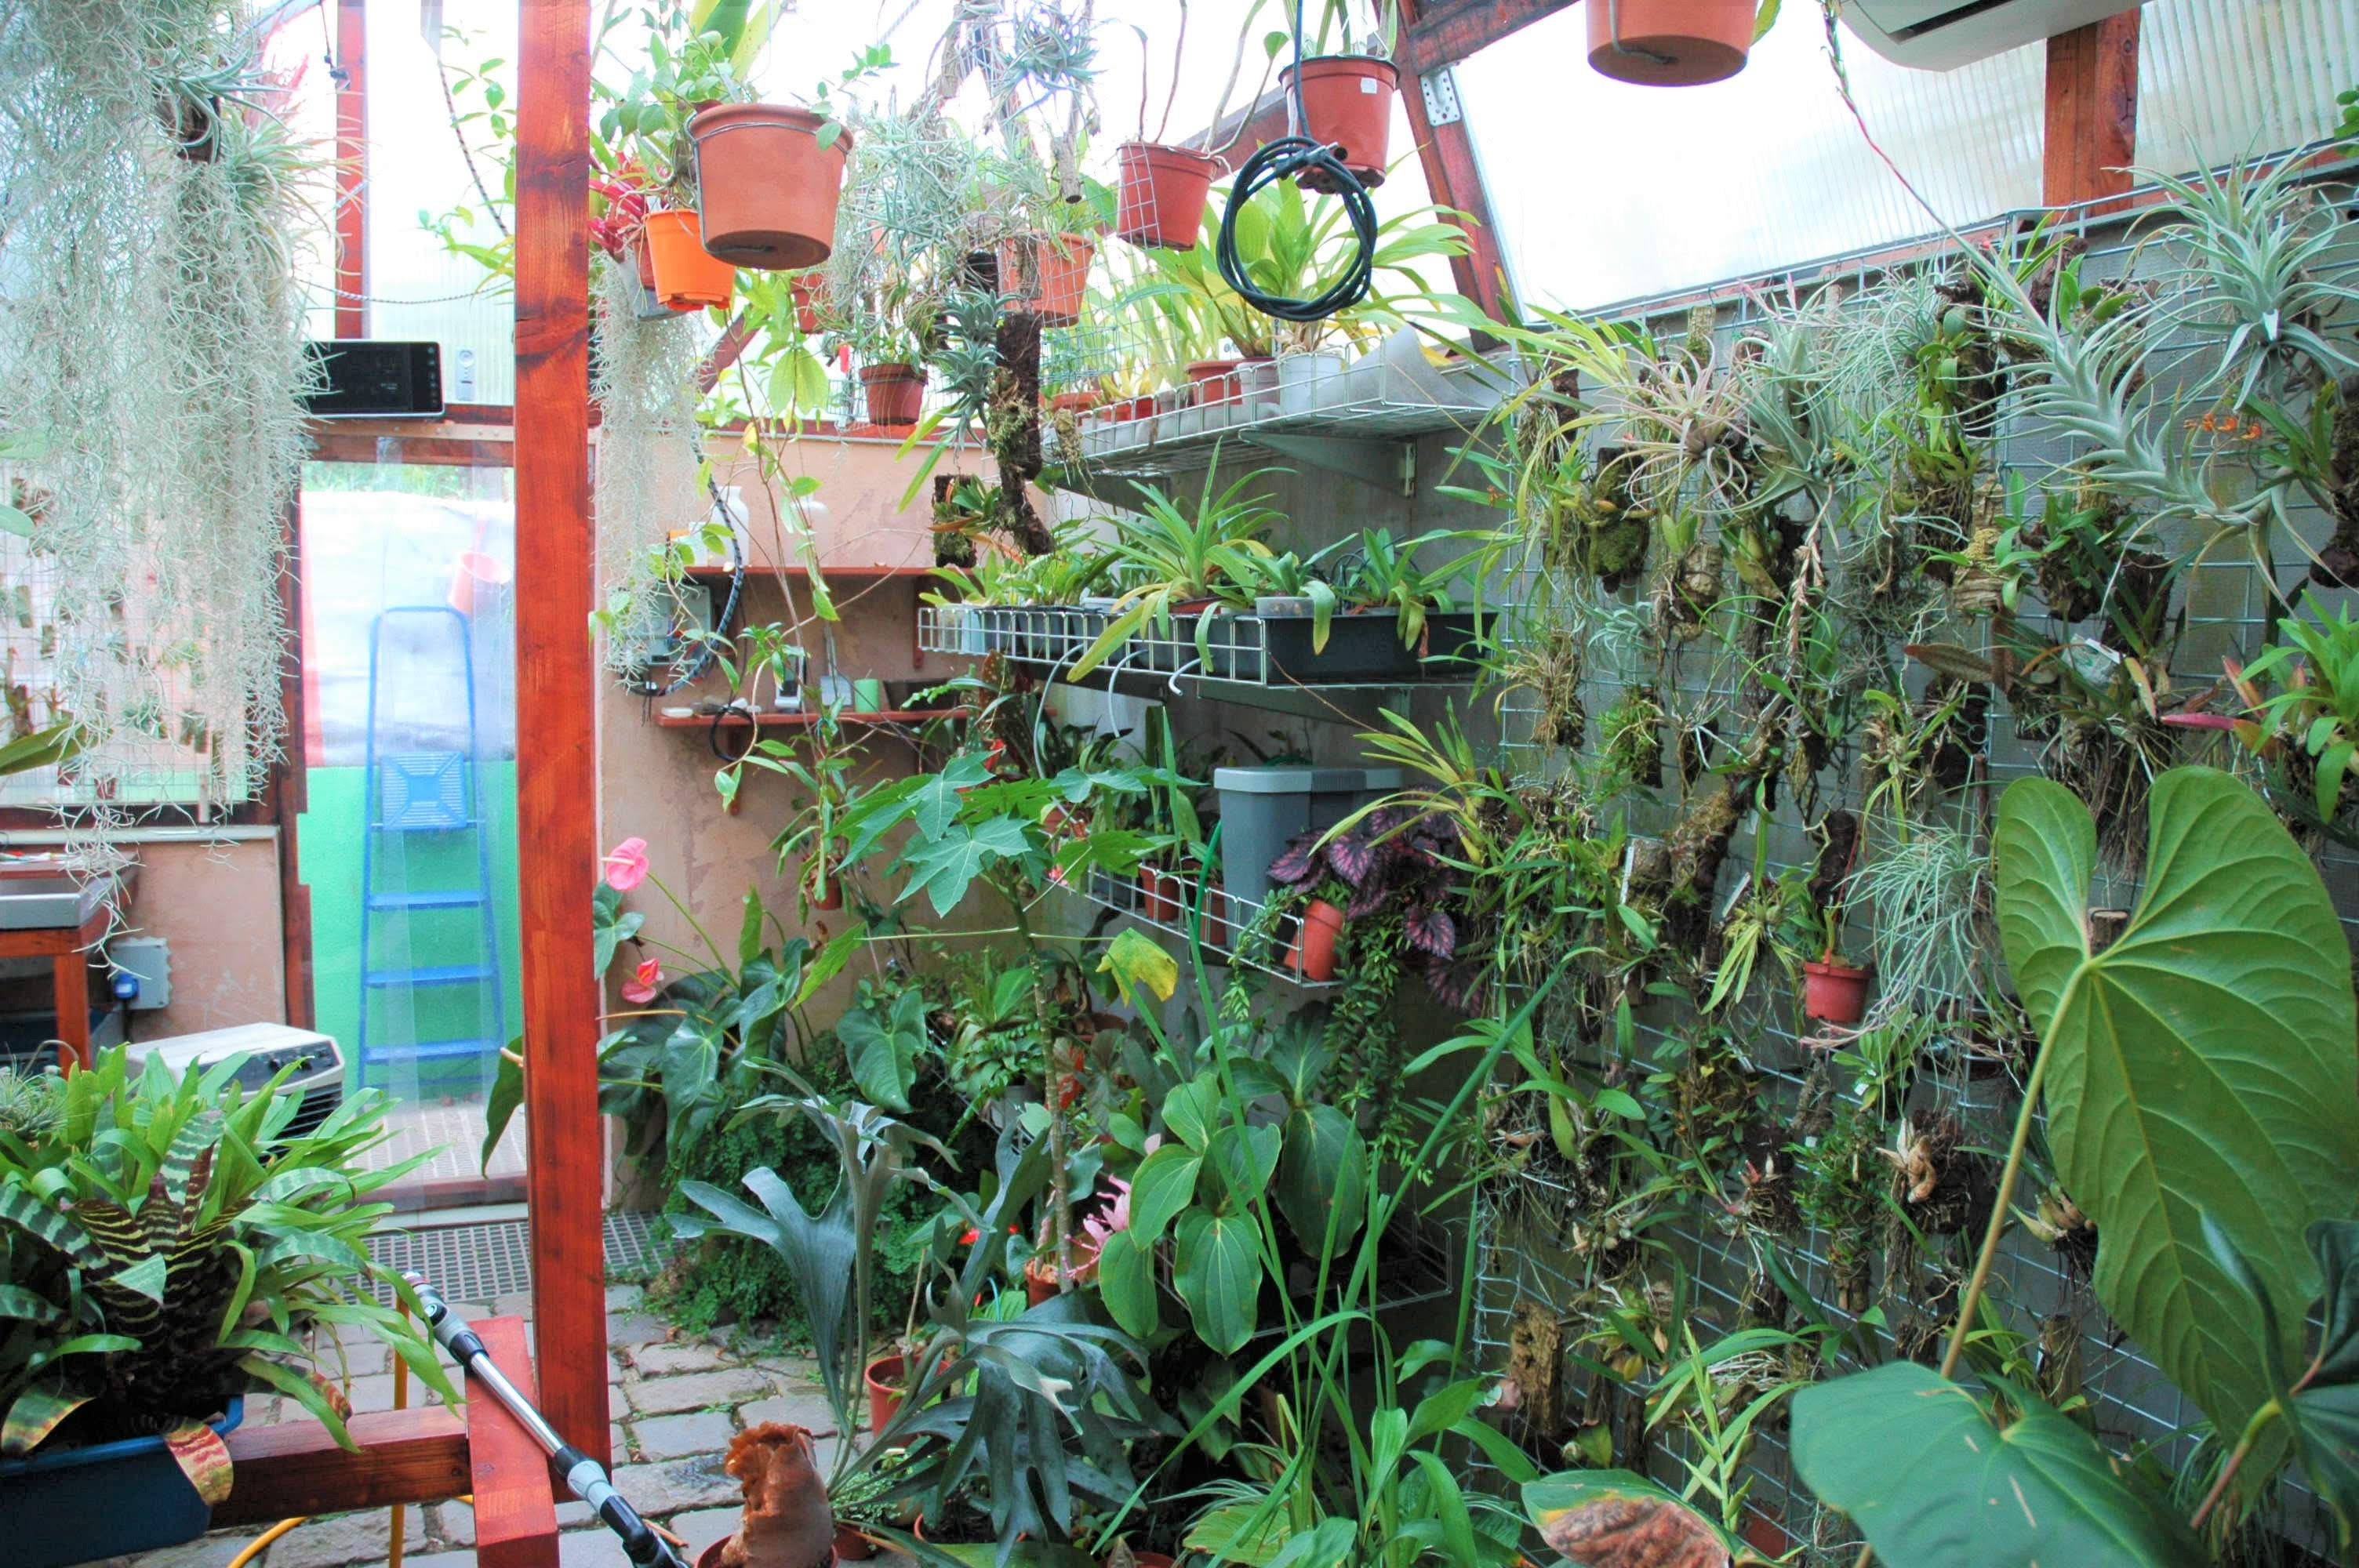
\includegraphics[width=\textwidth]{img/VS_5.jpg}
    \caption{Fotografie velkého skleníku}
    \label{fig:VS5} 
\end{figure}

\end{document}
